\section{Uso della probabilità negli algoritmi}
% pag 122

\subsection{Nell'analisi}
% pag 122

Nell'analisi probabilistica lo spazio di probabilità $\Omega$ che sottende l'analisi di probabilità non sono le scelte casuali fatte dall'algoritmo, perché l'algoritmo non ne fa, ma è uno spazio di probabilità sugli ingressi dell'algoritmo.

Se gli spazi di probabilità sono suddivisi rispetto alla taglia dell'input, $
\Omega_n
$ è uno spazio di probabilità su $
\bi{}_n
$, ovvero l'insieme delle istanze di taglia $n$.
\begin{equation*}
    \Omega_n
    =
    \bi{}_n
    =
    \left\{ 
        i \in \bi{} : |i| = n
    \right\}
\end{equation*}
Lo spazio delle probabilità sono tutte le possibili istanze, e ogni istanza ha una certa probabilità di accadere.
Si studia l'algoritmo deterministico su una particolare distribuzione degli ingressi.
Nel caso più semplice, la distribuzione è uniforme.

% A questo punto diventa tutto una variabile aleatoria.
Se si suppone di dover studiare l'algoritmo su un input estratto a caso, ci sono parecchie variabili aleatorie rilevanti.
In particolare, la probabilità di errore viene studiata in base all'istanza d'ingresso:
\begin{equation*}
    Pr \left( 
        \text{$A$ sia corretto su $
            \bm{i}
            , 
            |
            \bm{i}
            | = n$}
    \right)
\end{equation*}
E per esempio grazie a Pomerance, per il test di primalità vale 
$
\lim_{n \to \infty} p_n = 1
$.

Ci possono essere di casi in cui l'analisi probabilistica viene fatta sul tempo di esecuzione dell'algoritmo:
la performance al caso peggiore cerca l'istanza critica per cui l'algoritmo impiega più tempo, 
ma si può supporre che gli input siano estratti uniformemente dallo spazio delle istanze
e si vuole studiare l'algoritmo deterministico e la sua performance media su un input estratto casualmente dallo spazio.
\\
Anche la complessità diventa allora una variabile aleatoria, e si studia il comportamento di $
\bm{T}_A
$ su una certa istanza (anch'essa aleatoria) $
\bm{i}
$:
\begin{equation*}
    Pr \left( 
        \text{$
            \bm{T}_A \left( 
                \bm{i}
            \right)
            \leq f (n)
            , \,
            |
            \bm{i}
            | = n
        $}
    \right)
\end{equation*}
Che è una sorta di proprietà distribuzionale di $
\bm{T}_A \left( 
    \bm{i}
\right)
$.
\\
Per esempio, quicksort è un algoritmo deterministico, ma se lo si studia su sequenze scelte a caso, si dimostra che al caso medio ha complessità $
O \left( n \log n \right)
$ invece di $
O \left( n^2 \right)
$ che risulta avere al caso peggiore.

L'analisi al caso medio è proprio l'analisi probabilistica di un algoritmo deterministico.
Se $
\bm{i}_n
$ è un'istanza di taglia $n$ in $
\bi{}_n
$, la media del tempo di esecuzione su istanze $
\bm{i}_n
$ estratte a caso.
\begin{equation*}
    \E{
        T_A \left( 
            \bm{i}_n
        \right)
    }
\end{equation*}
Questa analisi fa un'assunzione molto forte, dovendo conoscere lo spazio di probabilità e la probabilità degli eventi elementari, che molto spesso si assume uniforme.
Se si deve estrarre un numero primo casuale questo è ragionevole, ma se per esempio si devono ordinare dati, l'assunzione sul loro ordinamento casuale è molto forte, e in genere non accurata, dato che in pratica i dati sono spesso già ordinati a gruppi.
La permutazione di ingressi quindi non è casuale, e in più quicksort (nella versione che sceglie il primo elemento come pivot) performa molto male su dati ordinati, rendendo l'analisi particolarmente inefficace.

\subsection{Nell'algoritmo}
% pag 122.7

Lo spazio di probabilità viene creato dall'algoritmo stesso:
l'insieme $
\Omega_n
$ è formato delle scelte casuali fatte dall'algoritmo.
Lo spazio non è basato sugli ingressi, perché in un algoritmo randomizzato si considera un ingresso fissato.
\begin{equation*}
    Pr \left( 
        \text{$A$ sia corretto su un input \emph{fissato}}
    \right)
\end{equation*}
Scelto un input, si studia la probabilità della corettezza al caso peggiore dell'algoritmo.
Si cerca quindi l'input su cui l'algoritmo sbaglia di più.

Anche in questo caso la  complessità può diventare una variabile aleatoria.
\begin{align*}
    Pr \left( 
        \bm{T}_A \left( 
            n
        \right)
        \geq c \cdot f(n)
    \right)
    &
    \leq d(n)
    \\
    Pr \left( 
        \bm{T}_A \left( 
            n
        \right)
        \leq c \cdot f(n)
    \right)
    &
    \geq d'(n)
\end{align*}
Per cui si studia la distribuzione del tempo di esecuzione.

\subsubsection{Algoritmi Las Vegas}
% pag 123
Gli algoritmi di tipo \emph{Las Vegas} sono algoritmi randomizzati \emph{sempre} corretti.
Dato un algoritmo $
A_{\bpi{}} \left( i \right) \to s
$, questo ritorna sempre la soluzione esatta.
\begin{equation*}
    Pr \left( 
        i
        \,
        \bpi{}
        \,
        s
    \right)
    = 1
\end{equation*}
La randomizzazione viene utilizzata per rendere aleatorio il tempo di esecuzione
\begin{align*}
    Pr \left( 
        \bm{T}_A \left( 
            n
        \right)
        \leq c \cdot f(n)
    \right)
    &
    \geq d(n)
\end{align*}
Esempi di algoritmi di questo tipo sono il quicksort randomizzato o gli algoritmi di approssimazione. Quest'ultimi ritornano una soluzione che può non essere ottima, ma è sempre ammissibile.

\subsubsection{Algoritmi Monte Carlo}
% pag 123.3
Gli algoritmi di tipo \emph{Monte Carlo} sono algoritmi randomizzati che \emph{possono} sbagliare.
Dato un algoritmo $
A_{\bpi{}} \left( i \right) \to s
$, si studia la sua probabilità di correttezza $
p_c(n)
$:
\begin{equation*}
    Pr \left( 
        i
        \,
        \bpi{}
        \,
        s
    \right)
    = p_c(n)
\end{equation*}
Anche per algoritmi di questo tipo si analizza il tempo di esecuzione
\begin{align*}
    Pr \left( 
        \bm{T}_A \left( 
            n
        \right)
        \leq c \cdot f(n)
    \right)
    &
    \geq d(n)
\end{align*}
e ci sono casi in cui questo è deterministico, perché il numero di iterazioni non è legato alle scelte casuali effettuate e vale $
d(n) = 1
$.

\subsubsection{Algoritmi Monte Carlo decisionali}
% pag 123.5
Gli algoritmi \emph{Monte Carlo} decisionali possono commettere errori di due tipi:
\begin{itemize}
    \item \emph{one-sided}: possono compiere errori solo su uno dei due \emph{outcome}
    \item \emph{two-sided}: possono compiere errori su entrambi gli \emph{outcome}
\end{itemize}

\subsection{Bound in alta probabilità}
% pag 123.8

\subsubsection{Limite alla complessità in alta probabilità}

\begin{definition}
    [Complessità in alta probabilità]
    \label{def:complessita_alta_prob}
    Dato $
    \bpi{} \subseteq \bi{} \times \bs{}
    $, un algoritmo randomizzato $
    A_{\bpi{}}
    $ ha complessità $
    O \left( f(n) \right)
    $ con alta probabilità se $
    \exists c, d > 0
    $ costanti, $
    \exists n_0
    $ tali che $
    \forall n \geq n_0, 
    \,
    \forall i \in \bi{}_n
    $ vale 
    \begin{equation*}
        Pr \left( 
            T \left( 
                A_{\bpi{}}
                (i)
            \right)
            \geq c f(n)
        \right)
        \leq
        \frac{1}{n^d}
    \end{equation*}
    o alternativamente
    \begin{equation*}
        Pr \left( 
            T \left( 
                A_{\bpi{}}
                (i)
            \right)
            \leq c f(n)
        \right)
        \geq
        1-
        \frac{1}{n^d}
    \end{equation*}
\end{definition}
Note:
\\
$d$ può essere una costante qualsiasi, anche minore di 1, perché è comunque sufficiente a indicare che c'è una sostanziale diminuzione della probabilità all'aumentare della taglia.
\\
Entrambi i metodi per definire l'alta probabilità delimitano la massa della probabilità della coda dell'istanza
\\
L'analisi è al caso peggiore: l'istanza non è scelta casualmente ma è fissata.
La probabilità invece è la probabilità sullo spazio $
\Omega_n
$ delle scelte fatte dall'algoritmo.

\subsubsection{Correttezza in alta probabilità}

\begin{definition}
    [Correttezza in alta probabilità]
    \label{def:correttezza_alta_prob}
    Dato $
    \bpi{} \subseteq \bi{} \times \bs{}
    $, un algoritmo randomizzato $
    A_{\bpi{}}
    $ è corretto in alta probabilità se $
    \exists d > 0
    $ costante, $
    \exists n_0
    $ tali che $
    \forall n \geq n_0, 
    \,
    \forall i \in \bi{}_n
    $ vale 
    \begin{equation*}
        Pr \left( 
            A_{\bpi{}}
            (i)
            \,
            \cancel{
                \bpi{}
            }
            \,
            i
        \right)
        \leq
        \frac{1}{n^d}
    \end{equation*}
\end{definition}
Note:
\\
È un'analisi di probabilità che mostra che l'algoritmo è corretto quasi sempre.
\\
È una caratterizzazione molto più forte della media: la massa di probabilità della coda della distribuzione ha misura che tende a 0.
\\
Il valore di $d$ può spesso essere aumentato molto con facilità: nel caso per esempio di Miller-Rabin, è sufficiente un valore delle iterazioni pari a 
\begin{equation*}
    s = \log_2 n
    \rightarrow
    Pr \left( errore \right)
    =
    \frac{1}{2^s}
    =
    \frac{1}{n}
\end{equation*}
per ottenere la correttezza in alta probabilità.
Aumentando di un fattore costante il numero di iterazioni la probabilità scende però esponenzialmente 
\begin{equation*}
    s = k \log_2 n
    \rightarrow
    Pr \left( errore \right)
    =
    \frac{1}{2^s}
    =
    \frac{1}{n^{k}}
\end{equation*}

\section{Concentration bound per variabili aleatorie}
% pag 124.3

\subsection{Disuguaglianze di Markov}
% pag 124.5
Per ogni variabile aleatoria intera positiva $
\bm{T}
$ vale $
\forall t
$:
\begin{equation*}
    Pr \left( 
        \bm{T} \geq t
    \right)
    \leq
    \frac{
        \E{
            \bm{T}
        }
    }{
        t
    }
\end{equation*}
Se in più $
\bm{T}
$ è limitata superiormente da $b$ con probabilità 1: $
Pr \left( \bm{T} > b \right) = 0
$ vale
\begin{equation*}
    \E{\bm{T}}
    \leq 
    t + 
    \left( 
        b - t
    \right)
    Pr \left( 
        \bm{T} \geq t
    \right)
\end{equation*}

\subsubsection{Confronto tra analisi al caso medio e in alta probabilità}

Se, come è ragionevole supporre in molti casi, l'algoritmo randomizzato ha limite superiore deterministico alla complessità al caso peggiore
\begin{equation*}
    Pr \left( 
        T_A(n) \leq cn^{\alpha}
    \right)
    = 1
\end{equation*}
(per esempio per quicksort randomizzato, anche nel caso peggiore di scelte più sfortunate, la complessità è al massimo quadratica.
Questa analisi lasca mette comunque un limite all'esecuzione, che non può diventare esponenziale).
\\
e si può scegliere $d = d_c$ come funzione crescente di $c$
(si può aumentare il grado del polinomio aumentando la constante moltiplicativa davanti alla complessità),
\begin{equation*}
    Pr \left( 
        T_A(n) \geq cf(n)
    \right)
    \leq
    \frac{1}{n^d}
\end{equation*}
sotto queste condizioni si dimostra che l'analisi al caso medio è meno informativa dell'analisi in alta probabilità.

Usando la seconda disuguaglianza di Markov con $
b = n^{\alpha}
$ e $
t = cf(n)
$, con $
c : d \geq \alpha
$:
\begin{align*}
    \E{
        \bm{T}_A (n)
    }
    &
    \leq
    c f(n)
    +
    \left( 
        n^{\alpha}
        -
        c f(n)
    \right)
    \frac{1}{n^d}
    \\
    &
    \leq
    c f(n)
    +
    \frac{n^{\alpha}}{n^d}
    \\
    &
    \leq
    c f(n)
    +
    1
\end{align*}

\subsection{Bound di Chernoff}
% pag 125.2

Data una generica famiglia di variabili indicatrici
\begin{equation*}
    X_i = 
    \begin{cases}
        1 & \text{con probabilità } p_i
        \\
        0 & \text{con probabilità } 1 - p_i
    \end{cases}
\end{equation*}
Le variabili sono mutualmente indipendenti, e vale $
\E{X_i} = p_i
$.
La variabile di interesse è la somma delle variabili indicatrici
\begin{equation*}
    X = 
    \sum_{i=1}^{n} X_i
\end{equation*}
Per cui vale \begin{equation*}
    \E{X}
    =
    \sum_{i=1}^{n} p_i
    =
    \mu
\end{equation*}

\begin{lemma}
    [Chernoff]
    \label{def:lemma_chernoff}
    Siano $
    X_1, \cdots, X_n
    $ variabili indicatrici con $
    p_i = Pr \left( X_i = 1 \right)
    $. Data $
    X = \sum_{i=1}^{n} X_i
    $ e $
    \mu
    =
    \E{X}
    =
    \sum_{i=1}^{n} p_i
    $, $
    \forall \delta > 0
    $ vale
    \begin{equation*}
        Pr \left( 
            X > \left( 1+ \delta \right) \mu
        \right)
        <
        \left( 
            \frac{
                e^{\delta}
            }{
                \left( 
                    1 + \delta
                \right)^{
                    \left( 
                        1 + \delta
                    \right)
                }
            }
        \right)^{\mu}
    \end{equation*}
\end{lemma}
Note:
\\
Questo lemma fornisce un bound molto più stretto di Markov, infatti 
la frazione è un numero minore di 1 ($
    \left( 
        1 + \delta
    \right)^{
        \left( 
            1 + \delta
        \right)
    }
$ cresce molto più velocemente di $
e^\delta
$) e 
$\mu$ è legato al numero di variabili indicatrici,
quindi c'è un bound esponenziale,
mentre la prima disuguaglianza di Markov risulta
\begin{equation*}
    Pr \left( 
        X > \left( 1+ \delta \right) \mu
    \right)
    < 
    \frac{\mu}{
        \left( 
            1 + \delta
        \right)
        \mu
    }
    =
    \frac{1}{
        1 + \delta
    }
\end{equation*}
che non ha alcun legame con la taglia.
% I bound di \emph{Chernoff} sono più stretti di quelli di Markov, ma valgono solo per variabili aleatorie particolari.

\begin{proof}
    Si considera la famiglia di variabili aleatorie
    \begin{equation*}
        Y_t = e^{tX}
    \end{equation*}
    e ne si studia la media per trovarne una correlazione con la media di $X$.
    Per prima cosa si mostra che
    \begin{align*}
        \E{
            e^{t X}
        }
        &= 
        \E{
            e^{
                t
                \sum_{i=1}^{n} X_i
            }
        }
        \\
        &= 
        \E{
            e^{
                \sum_{i=1}^{n} t X_i
            }
        }
        \\
        &= 
        \E{
            \prod_{i=1}^{n}
            e^{
                t X_i
            }
        }
        \intertext{le variabili $e^{t X_i} $ sono indipendenti, perché le $X_i$ sono indipendenti e la funzione è invertibile, per cui la media del prodotto è il prodotto delle medie}
        &= 
        \prod_{i=1}^{n}
        \E{
            e^{
                t X_i
            }
        }
        \intertext{vale per una singola variabile $
            \E{
                e^{t X_i}
            }
            = 
            e^{t \cdot 0}
            \left( 1 - p_i \right)
            +
            e^{t \cdot 1}
            p_i
            =
            1 + p_i \left( e^t - 1 \right)
            $
        }
        &= 
        \prod_{i=1}^{n}
        \left( 
            1 + p_i \left( e^t - 1 \right)
        \right)
        \intertext{considerando la serie di Taylor troncata vale $
            e^y > 1+y
        $}
        &<
        \prod_{i=1}^{n}
        e^{
            p_i \left( e^t - 1 \right)
        }
        \\
        &= 
        e^{
            \sum_{i=1}^{n}
            p_i \left( e^t - 1 \right)
        }
        \\
        &= 
        e^{
            \left( e^t - 1 \right)
            \sum_{i=1}^{n}
            p_i
        }
        \\
        &= 
        e^{
            \left( e^t - 1 \right)
            \mu
        }
    \end{align*}
    Si sfrutta questo risultato per provare il lemma
    \begin{align*}
        Pr \left( 
            X > \left( 1 + \delta \right) \mu
        \right)
        &= 
        Pr \left( 
            tX > t \left( 1 + \delta \right) \mu
        \right)
        \\
        &= 
        Pr \left( 
            e^{
                tX
            }
            >
            e^{
                t \left( 1 + \delta \right) \mu
            }
        \right)
        \\
        &= 
        Pr \left( 
            Y_t
            >
            e^{
                t \left( 1 + \delta \right) \mu
            }
        \right)
        \intertext{e per la prima disuguaglianza di Markov}
        &< 
        \frac{
            \E{
                Y_t
            }
        }{
            e^{
                t \left( 1 + \delta \right) \mu
            }
        }
        \\
        &= 
        \frac{
            \E{
                e^{tX}
            }
        }{
            e^{
                t \left( 1 + \delta \right) \mu
            }
        }
        \intertext{e per il risultato precedente}
        &<
        \frac{
            e^{
                \left( e^t - 1 \right)
                \mu
            }
        }{
            e^{
                t \left( 1 + \delta \right) \mu
            }
        }
        \intertext{questa è una famiglia di limiti superiori, valida $\forall t > 0$, di cui si seleziona il più stretto che risulta: $
            t_{min} =
            \ln \left( 1 + \delta \right)
            $
        }
        &<
        \frac{
            e^{
                \left(
                    e^{
                        \ln \left( 1 + \delta \right)
                    }
                - 1 \right)
                \mu
            }
        }{
            e^{
                \ln \left( 1 + \delta \right)
                \left( 1 + \delta \right) \mu
            }
        }
        \intertext{chiaramente $
            e^{
                \ln \left( 1 + \delta \right)
            }
            =
            \left( 1 + \delta \right)
            $
        }
        &= 
        \frac{
            e^{
                \left( 
                    1 + \delta - 1
                \right)
                \mu
            }
        }{
            \left( 1 + \delta \right)^{
                \left( 1 + \delta \right) \mu
            }
        }
        \intertext{numeratore e denominatore sono elevati alla $\mu$, e si conclude}
        &= 
        \left( 
            \frac{
                e^{\delta}
            }{
                \left( 
                    1 + \delta
                \right)^{
                    \left( 
                        1 + \delta
                    \right)
                }
            }
        \right)^{\mu}
    \end{align*}
\end{proof}

\begin{corollario}
    Per $
    0 < \delta < 1
    $ valgono i seguenti bound
    \begin{align*}
        Pr \left( 
            X > \left( 1 + \delta \right) \mu
        \right)
        &
        <
        e^{
            -\delta^2 \mu / 3
        }
        \\
        Pr \left( 
            X < \left( 1 - \delta \right) \mu
        \right)
        &
        <
        e^{
            -\delta^2 \mu / 2
        }
    \end{align*}
\end{corollario}
Per cui i valori di $X$ sono estremamente concentrati intorno alla media.
Se si ricava un valore di $d$ per cui $
\delta^2 \mu / 2
> 
d \log n
$ si ottiene l'alta probabilità
\begin{equation*}
    Pr \left( 
        X < \left( 1 - \delta \right) \mu
    \right)
    <
    e^{
        -\delta^2 \mu / 2
    }
    <
    \frac{1}{n^d}
\end{equation*}
Se quello scostamento dalla media rappresenta l'evento ``cattivo'', in questo modo si riesce a limitare la probabilità della sua occorrenza con un inverso di un polinomio in $n$.

\section{Analisi di Quicksort randomizzato}
% pag 128

\subsection{Implementazione}
% pag 128

L'algoritmo di quicksort viene definito su un insieme $S$ di elementi distinti. Questo non comporta perdita di generalità, perché eventuali chiavi ripetute si possono arricchire con la posizione iniziale nella lista per sciogliere i conflitti.

Si definiscono gli elementi ordinati come \emph{order statistics}:
\begin{equation*}
    \Call{Sort}{S}
    =
    \langle x_1, \cdots, x_n \rangle
\end{equation*}

L'algoritmo è quello standard:
\begin{algorithm}[H]
\caption{Template per Quicksort}\label{alg:quicksort}
\begin{algorithmic}[1]
    \Procedure{Quicksort}{$S$}
        \If{$|S| \leq 1$}
        \Comment{BASE}
            \State return $S$
        \EndIf
        \State $y \gets 
            \Call{Choose\_Pivot}{S}
        $
        \label{alg:quicksort:choose}
        \Comment{DIVIDE}
        \State $S_1 \gets \left\{ 
            s \in S : s < y
        \right\}
        $
        \State $S_2 \gets \left\{ 
            s \in S : s > y
        \right\}
        $
        \State $X_1 \gets 
            \Call{Quicksort}{S_1}
        $
        \Comment{RECURSE}
        \State $X_2 \gets 
            \Call{Quicksort}{S_2}
        $
        \State return $\langle X_1, y, X_2 \rangle$
        \Comment{CONQUER}
    \EndProcedure
\end{algorithmic}
\end{algorithm}
\noindent
Alla riga \ref{alg:quicksort:choose} si effettua la scelta del pivot, che comporta versioni diverse dell'algoritmo.
Il costo del divide non è trascurabile, in particolare alcuni tipi di scelta sono molto costosi, ma in ogni caso lineari nella taglia. Anche la divisione in insiemi è lineare. Il conquer ha costo fisso.

L'albero delle ricorsioni ha struttura simile a prescindere dalla scelta.
\begin{figure}[h]
    \centering
    \caption{Albero delle ricorsioni di Quicksort}
    \label{fig:qs_rec_tree}
    \begin{tikzpicture} [
            scale=1.2,
            % nodo/.style={ellipse,fill=black!25,minimum size=20pt,inner sep=0pt},
            nodo/.style={circle,fill=black!25,minimum size=25pt,inner sep=0pt},
            arco/.style = {draw,thin,-},
            % outbound edge/.style = {draw,line width=4pt,-,blue!30},
            % selected edge/.style = {draw,line width=4pt,-,red!30},
        ]
        % First we draw the vertices
        \foreach \pos/\name/\labin/\labout in {
                {(0,5)/a/S/n=|S|},
                {(-2,4)/b/S_1/c|S_1|},
                {(2,4)/c/S_2/c|S_2|}}
                % {(-3,3)/d/S_{11}/|S_{11}|},
                % {(-1,3)/e/S_{12}/|S_{12}|},
                % {(1,3)/f/S_{21}/|S_{21}|},
                % {(3,3)/g/S_{22}/|S_{22}|}}
            \node[nodo, label={$\labout$}] (\name) at \pos {$\labin$};
        % \foreach \pos/\name/\labin in {
                % {(0,5)/a/S},
                % {(-2,4)/b/S_1},
                % {(2,4)/c/S_2},
                % {(-3,3)/d/S_{11}},
                % {(-1,3)/e/S_{12}},
                % {(1,3)/f/S_{21}},
                % {(3,3)/g/S_{22}}}
            % \node[nodo] (\name) at \pos {$\labin$};
        \foreach \source/ \dest in {
                % b/d,b/e,
                % c/f,c/g,
                a/b,a/c}
            \path[arco] (\source) -- (\dest);
        \begin{pgfonlayer}{background}
        \end{pgfonlayer}
    \end{tikzpicture}
\end{figure}
Ad ogni livello, $S_1$ e $S_2$ sono una \emph{sottopartizione} di $S$, quindi la somma delle taglie è minore di $n$ ad ogni livello:
$
\sum |S_j^l| \leq n
$, e ogni livello non può eseguire più di $cn$ lavoro.
Allora, se $h$ è l'altezza massima dell'albero delle chiamate, il tempo di esecuzione è limitato da
\begin{equation*}
    T_{QS} (n) \leq cnh
\end{equation*}
L'altezza $h$ dipende dalla scelta del pivot eseguita.

\subsubsection{Scelta del primo elemento come pivot}

Se la scelta del pivot viene implementata come
\begin{algorithmic}[1]
    \Procedure{Choose\_Pivot}{$S$}
        \State return $s_1$
    \EndProcedure
\end{algorithmic}
il caso peggiore avviene quando l'insieme è già ordinato. In questa situazione, $
S_1 = \emptyset
$ e $
S_2 = S - \left\{ s_1 \right\}
$.
\begin{figure}[h]
    \centering
    \caption{Albero delle ricorsioni nel caso peggiore}
    \label{fig:qs_rec_tree_bad}
    \begin{tikzpicture} [
            scale=1.2,
            nodo/.style={ellipse,fill=black!25,minimum size=20pt,inner sep=0pt},
            % nodo/.style={circle,fill=black!25,minimum size=25pt,inner sep=0pt},
            arco/.style = {draw,thin,-},
            arco tratteggiato/.style = {draw,thin,dotted},
            % outbound edge/.style = {draw,line width=4pt,-,blue!30},
            % selected edge/.style = {draw,line width=4pt,-,red!30},
        ]
        % First we draw the vertices
        \foreach \pos/\name/\labin/\labout in {
                {(0,5)/a/n/cn},
                {(-2,4)/b/\emptyset/0},
                {(2,4)/c/n-1/c(n-1)},
                {(1,3)/f/\emptyset/0},
                {(4,2)/g/1/0}}
            \node[nodo, label={$\labout$}] (\name) at \pos {$\labin$};
            % \node[nodo, label={$\labout$}] (\name) at \pos {\name $\labin$};
        \foreach \source/ \dest in {
                c/f,
                a/b,a/c}
            \path[arco] (\source) -- (\dest);
        \foreach \source/ \dest in {
                c/g}
            \path[arco tratteggiato] (\source) -- (\dest);
        \begin{pgfonlayer}{background}
        \end{pgfonlayer}
    \end{tikzpicture}
\end{figure}
Sommando tutti i work eseguiti nell'albero in \rfig{fig:qs_rec_tree_bad} si ottiene
\begin{equation*}
    T_{QSfirst} (n) = c \frac{n(n-1)}{2}
    =
    \Theta \left( cn^2 \right)
\end{equation*}

\subsubsection{Scelta della mediana come pivot}

Se la scelta del pivot viene implementata come
\begin{algorithmic}[1]
    \Procedure{Choose\_Pivot}{$S$}
        \State return $x_{
            \left\lfloor 
            n/2
            \right\rfloor
            +1
        }$
    \EndProcedure
\end{algorithmic}
Dove viene ritornata l'order statistic centrale,
si ottiene l'albero più bilanciato possibile, dove la taglia dell'insieme dimezza ad ogni livello.
Ci sono quindi $
h = \log n
$ livelli, per una complessità pari a 
\begin{equation*}
    T_{QSmedian} (n) \leq cnh = O \left( n \log n \right)
\end{equation*}
Selezionare la mediana però è molto costoso, esiste un algoritmo deterministico lineare per calcolarla, ma la costante è molto alta (circa $80n$), ed è quindi inutilizzabile in pratica.

\subsection{Scelta casuale del Pivot}
% pag 129.5

\subsubsection{Profondità dell'albero}

Supponendo di riuscire a garantire una taglia degli insiemi generati limitata da
\begin{equation*}
    |S_1|, |S_2| \leq \frac{3}{4} t
\end{equation*}
e ricordando il legame tra le taglie, un limite superiore implica anche un limite inferiore:
\begin{equation*}
    |S_1| = n - 1 - |S_2|
\end{equation*}
In questo caso, la taglia del primo livello è
\begin{align*}
    |S_0| &= n
    \\
    |S_{i+1}|
    &\leq
    \frac{3}{4} |S_{i}|
    \intertext{per unfolding: }
    |S_{i}|
    &\leq
    \left( 
        \frac{3}{4}
    \right)^i
    |S|
    = 
    \left( 
        \frac{3}{4}
    \right)^i
    n
\end{align*}
La taglia allora decresce esponenzialmente, e il numero di livelli risulta
\begin{equation*}
    h = O \left( \log_{4/3} n \right)
\end{equation*}

\subsubsection{Scelta casuale del pivot}

La scelta casuale del pivot riesce a garantire questa proprietà delle taglie dei sottoinsiemi in alta probabilità.
\begin{algorithmic}[1]
    \Procedure{Choose\_Pivot}{$S$}
        \State return $\Call{Random}{S}$
    \EndProcedure
\end{algorithmic}
Si consideri l'insieme degli elementi ``fortunati''
\begin{equation*}
    F = 
    \left\{ 
        X_i
        % \quad 
        % \text{con}
        % \quad 
        :
        i \in
        \left\{ 
            \left\lfloor 
            \frac{n}{4} + 1
            \right\rfloor
            , \cdots , 
            \left\lceil 
            \frac{3}{4}n + 1
            \right\rceil
        \right\}
    \right\}
\end{equation*}
Questo insieme contiene circa la metà degli elementi, per cui la probabilità di selezionare un elemento in questo insieme è circa un mezzo.
\\
Se viene scelto come pivot un elemento di questo insieme, entrambi i sottoinsiemi hanno taglia inferiore ai $3/4$ dell'insieme originale, infatti, il primo insieme deve contenere almeno il primo quarto degli elementi
\begin{equation*}
    |S_1| \geq
    \left\lfloor 
        \frac{n}{4} + 1
    \right\rfloor
    \quad
    \rightarrow
    \quad
    |S_2| \leq
    n - 1 -
    \left\lfloor 
        \frac{n}{4} + 1
    \right\rfloor
    \leq
    \frac{3}{4} n
\end{equation*}
e analogamente, il secondo insieme deve contenere almeno l'ultimo quarto di elementi
\begin{equation*}
    |S_2| \geq
    n -
    \left\lceil 
    \frac{3}{4}n
    \right\rceil
    \quad
    \rightarrow
    \quad
    |S_1| \leq n - 1 - \left( 
        n -
        \left\lceil 
        \frac{3}{4}n
        \right\rceil
    \right)
    \leq
    \frac{3}{4}n
\end{equation*}
Per cui nel corso delle scelte del pivot, circa una volta su due viene effettuata una scelta fortunata.
L'intuizione è che in media, un cammino non potrà essere lungo più di due volte il cammino più corto possibile.
Lungo un cammino da radice a foglia, un nodo su due garantisce una riduzione di $3/4$ della taglia dell'insieme.
Questo garantisce un numero logaritmico di livelli, che corrisponde a un algoritmo $n \log n$ con alta probabilità, con una scelta del pivot che si può realizzare in tempo costante.

\subsubsection{Analisi della profondità}

Fissato $
t = a \log_{4/3} n
$ come target di altezza dell'albero,
si vuole determinare la probabilità dell'evento negativo
\emph{any bad path}
\begin{equation*}
    ABP = 
    \text{un arbitrario cammino è lungo più di $a \log_{4/3} n$}
\end{equation*}
Riguardo al numero di cammini distinti,
se nell'albero delle ricorsioni si eliminano gli insiemi vuoti,
ne esiste uno per foglia dell'albero, ed è presente una foglia per ogni elemento.
Ci sono allora $n$ cammini radice-foglia nell'albero, ciascuno individuato da un valore $x_i$.
Si studia allora la probabilità dell'evento \emph{fixed bad path}, per un cammino fissato:
\begin{align*}
    FBP = 
    &
    \;
    \text{un cammino \emph{fissato} da radice a foglia nell'albero}
    \\
    &
    \;
    \text{della ricorsione ha profondità maggiore di $a \log_{4/3} n$}
\end{align*}
Se si conosce la probabilità per un cammino fissato,
si limita facilmente la probabilità che \emph{nessun} cammino sia più lungo di $t$ sfruttando l'\emph{union bound}.
Infatti, una volta nota la probabilità su un singolo evento negativo, la probabilità che un \emph{qualche} cammino sia molto lungo è minore o uguale alla somma delle probabilità associate a ogni singolo cammino.
Con lo \emph{union bound} si ricava quindi la probabilità che l'evento negativo \emph{Any Bad Path} accada.

% Si vuole studiare la lunghezza di un cammino fissato, non un cammino casuale generico.
Perché capiti l'evento ``cammino più lungo di $t$'', nei primi $
a
\log_{4/3} n
$ nodi del cammino, devono verificarsi \emph{meno} di $
\log_{4/3} n
$ scelte fortunate del pivot.
% Per assurdo
Infatti, ogni scelta fortunata abbassa di $3/4$ gli elementi, per cui dopo $
\log_{4/3} n
$ si sarebbe arrivati alla foglia. Ma il cammino in considerazione \emph{non} era terminato, quindi devono essere capitate meno di $
\log_{4/3} n
$ scelte fortunate.
\\
Questo si formalizza utilizzando le variabili indicatrici
\begin{equation*}
    X_i = 
    \begin{cases}
        1 & \text{scelta fortunata al livello $i$}
        \\
        0 & \text{altrimenti}
    \end{cases}
\end{equation*}
Le scelte ad ogni livello sono chiaramente indipendenti,
e vale 
\begin{equation*}
    Pr \left( X_i = 1 \right) \geq \frac{1}{2}
\end{equation*}
Si può allora studiare la somma nei primi $t$ livelli dell'albero, che rappresenta il numero di scelte fortunate compiute
\begin{equation*}
    X = \sum_{i=1}^{a \log_{4/3} n} X_i
    \quad
    \rightarrow
    \quad
    \mu = \E{X} = \frac{1}{2} a \log_{4/3} n = \frac{t}{2}
\end{equation*}
Per applicare il bound di Chernoff, va riscritto il vincolo su $X$ in funzione di $\delta < 1$ e $\mu$
\begin{equation*}
    Pr \left( 
        X < \log_{4/3} n
    \right)
    \quad
    \leftrightarrow
    \quad
    Pr \left( 
        X < \left( 1 - \delta \right) \mu
    \right)
\end{equation*}
I valori corretti sono $a=8$ e $\delta=3/4$, ottenuti portando avanti l'analisi simbolica, e ricavando il valore necessario in modo che
\begin{align*}
    t = 8 \log_{4/3} n
    \quad
    &
    \rightarrow
    \quad
    \mu = 4 \log_{4/3} n 
    \\
    \delta = \frac{3}{4}
    \quad
    &
    \rightarrow
    \quad
    1 - \delta = \frac{1}{4}
    \\
    \left( 1 - \delta \right) \mu &= \log_{4/3} n
\end{align*}
Si può quindi procedere applicando il corollario del lemma di Chernoff
\begin{align*}
    Pr \left( 
        X < \log_{4/3} n
    \right)
    &= 
    Pr \left( 
        X
        <
        \left( 1 - \frac{3}{4} \right) 4
        \log_{4/3} n
    \right)
    \\
    &
    \leq
    e^{
        - \left( 
            \frac{3}{4}
        \right)^{2}
        4
        \log_{4/3} n
        \big/ 2
    }
    \\
    &= 
    e^{
        - \frac{9}{8}
        \log_{4/3} n
    }
    \\
    &
    <
    e^{
        - \log_{4/3} n
    }
    \\
    &= 
    e^{
        - \ln n / \ln (4/3)
    }
    \\
    &= 
    \frac{1}{
        n^{
            \frac{
                1
            }{
                \ln (4/3)
            }
        }
    }
    \\
    &
    \approx
    \frac{1}{
        n^{
            3,47
        }
    }
    \\
    &
    <
    \frac{1}{n^3}
\end{align*}
Riassumendo, l'evento ``cattivo'' per cui l'albero ha altezza maggiore di $a \log_{4/3} n$ accade con probabilità
\begin{align*}
    Pr
    &
    \left( 
        \text{l'albero ha altezza $> 8 \log_{4/3} n$}
    \right)
    \leq
    \\
    &
    =
    Pr \left( 
        % \text{\emph{Any Bad Path}}
        \text{esiste \emph{un} cammino di lunghezza $> 8 \log_{4/3} n$}
    \right)
    \\
    &
    \leq
    n
    Pr \left( 
        % \text{\emph{Fixed Bad Path}}
        \text{un cammino \emph{fissato} ha lunghezza $> 8 \log_{4/3} n$}
    \right)
    \\
    &
    \leq
    n
    Pr
    \left( 
        \text{ci sono meno di $\log_{4/3} n$ scelte fortunate}
    \right.
    \\
    &
    \quad
    \quad
    \quad
    \quad
    \left.
        \text{nei primi $a \log_{4/3} n$ nodi del cammino}
    \right)
    \\
    &
    \leq
    n
    \frac{1}{n^3}
    =
    \frac{1}{n^2}
\end{align*}
Per cui in alta probabilità l'albero della ricorsione di quicksort randomizzato ha un numero logaritmico di livelli,
e ogni livello contribuisce al lavoro complessivo $
O (n)
$, per cui in alta probabilità quicksort esegue in tempo $
O (n \log n)
$.

Per gli algoritmi randomizzati si scompone l'analisi in una serie di eventi che possono accadere o meno,
e poi si studia l'evento buono (o cattivo) in funzione di questi singoli eventi elementari 
che catturano le varie scelte fatte dall'algoritmo.
L'analisi deterministica è simile, si scompone l'algoritmo in passi elementari e si trova qual è la sequenza peggiore.
Piuttosto che il caso peggiore, qua si studia la probabilità che questo avvenga,
scomponendo l'intera computasione in una serie di eventi da comporre tra di loro in maniera da poter usare i bound noti.

\subsubsection{Analisi al caso medio}

Utilizzando la disuguaglianza di Markov si passa facilmente dall'alta probabilità al caso medio.

La variabile $
T(n)
$ che rappresenta il tempo di quicksort randomizzato è limitata
\begin{equation*}
    Pr \left( 
        T(n) 
        \leq
        n^2
    \right)
    = 1
\end{equation*}
perché anche nel caso di scelte sempre sfortunate, termina in tempo quadratico. Il bound in alta probabilità è noto
\begin{equation*}
    Pr \left( 
        T(n)
        \geq
        8 n \log_{4/3} n
    \right)
    <
    \frac{1}{n^2}
\end{equation*}
per cui si può applicare la disuguaglianza di Markov per variabili limitate con $
b = n^2
$ e $
t = 
8 n \log_{4/3} n
$
\begin{align*}
    \E{T}
    &
    <
    t + \left( b-t \right) Pr \left( T > t \right)
    \\
    &= 
    8 n \log_{4/3} n
    +
    \left( 
        n^2
        -
        8 n \log_{4/3} n
    \right)
    \frac{1}{n^2}
    \\
    &<
    8 n \log_{4/3} n
    +1
\end{align*}

L'analisi randomizzata si può stringere molto, e risulta quasi lineare in $
n \log n
$.

In pratica quicksort è uno degli algoritmi di sorting più efficienti: la scelta del pivot è molto semplice, e anche la partizione può essere effettuata in maniera veloce.
Non si usa solo nei sistemi con cache molto profonde, dove \emph{k-way merge sort} riesce a sfruttare meglio la cache, generando meno miss.

\section{Amplificazione della probabilità}
% pag 132.6

Si consideri un algoritmo \emph{Monte Carlo} decisionale $
A_{\bpi{}}
$, che compie \emph{two-sided error}, caratterizzato da
\begin{equation*}
    Pr \left( 
        i
        \,
        \bpi{}
        \,
        A_{\bpi{}}
    \right)
    =
    \frac{1}{2} + \varepsilon
    \quad
    \text{con}
    \quad
    0 < \varepsilon \leq \frac{1}{2}
\end{equation*}
Questa minima deviazione dalla scelta casuale è sufficiente per costruire un algoritmo decisionale di precisione arbitraria: secondo il \emph{majority protocol}, si possono compiere un numero dispari di esecuzioni dell'algoritmo, e scegliere come corretta la risposta che viene restituita il numero maggiore di volte.
Si applica quindi un algoritmo deterministico su una \emph{black box} randomizzata.

\begin{algorithm}[H]
\caption{Majority protocol per amplificare la probabilità}\label{alg:maj_prot}
\begin{algorithmic}[1]
    \Procedure{M\_A}{$i, k$}
        \State $\mathit{ANS}[0] \gets 0 $
        \State $\mathit{ANS}[1] \gets 0 $
        \For{$i \gets 1 $ to $ 2k-1 $ }
            \State $r \gets A_{\bpi{}}(i)$
            \State $
            \mathit{ANS}[r]
            \gets 
            \mathit{ANS}[r] + 1
            $
        \EndFor
        \If{$\mathit{ANS}[0] \geq k$}
            \State return $\mathit{ANS}[0]$
        \Else
            \State return $\mathit{ANS}[1]$
        \EndIf
    \EndProcedure
\end{algorithmic}
\end{algorithm}
\noindent
La probabilità di errore $
Pr \left( 
    i
    \,
    \cancel{
        \bpi{}
    }
    \,
    \mathit{MA}_{\bpi{}}
\right)
$ si studia con la famiglia di variabili indicatrici 
\begin{equation*}
    X_i = 
    \begin{cases}
        1 & \text{se $i$-esima iterazione ha risultato corretto}
        \\
        0 & \text{altrimenti}
    \end{cases}
\end{equation*}
con chiaramente probabilità di successo della singola iterazione pari a 
\begin{equation*}
    Pr \left( 
        X_i = 1
    \right)
    =
    \frac{1}{2} + \varepsilon
\end{equation*}
di cui si studia la somma
\begin{equation*}
    X = \sum_{i=1}^{2k-1} X_i
    = \text{\# esecuzioni corrette di $
        A_{\bpi{}}
    $ all'interno di $
        \mathit{MA}_{\bpi{}}
    $}
\end{equation*}
e l'algoritmo $
    \mathit{MA}_{\bpi{}}
$ è corretto quando $
X \geq k
$.
La media di $X$ vale
\begin{equation*}
    \mu
    = \E{X}
    = 
    \left( 2k - 1 \right)
    \left(
        \frac{1}{2}
        + \varepsilon
    \right)
    =
    k - 
    \frac{1}{2}
    + 2k\varepsilon - \varepsilon
\end{equation*}
Per poter studiare $
Pr \left( 
    X < k
\right)
$ con i lemmi di Chernoff, occorre riscrivere $k$ in funzione di $\mu$ e $\delta$, in modo che $
Pr \left( 
    X < \left( 1 - \delta \right) \mu
\right)
$.
\begin{align*}
    k
    &= 
    \mu +
    \frac{1}{2}
    + \varepsilon -2k\varepsilon
    \intertext{vale $2k\varepsilon \geq \varepsilon \mu$: }
    &
    \qquad
    \qquad
    \begin{aligned}[t]
        \varepsilon \mu
        &= 
        \varepsilon 
        \left( 2k - 1 \right)
        \left( 
            \frac{1}{2}
            + \varepsilon
        \right)
        \\
        &= 
        \left( 2k - 1 \right)
        \left( 
            \frac{\varepsilon}{2}
            + \varepsilon^2
        \right)
        \\
        &
        \text{per $0 < \varepsilon \leq 1/2$ vale $\varepsilon^2 \leq \varepsilon/2$}
        \\
        &
        \leq
        2k
        \left( 
            \frac{\varepsilon}{2}
            +
            \frac{\varepsilon}{2}
        \right)
        = 2k\varepsilon
    \end{aligned}
    \\
    &
    \leq
    \mu +
    \frac{1}{2} + \varepsilon
    - \varepsilon \mu
    \\
    &
    \leq
    \mu - \varepsilon \mu + 1
    \\
    &
    \leq
    \left( 1 - \varepsilon \right) \mu + 1
\end{align*}
Per cui risulta
\begin{align*}
    Pr \left( 
        i
        \,
        \cancel{
            \bpi{}
        }
        \,
        \mathit{MA}_{\bpi{}}
    \right)
    &= 
    Pr \left( 
        X < k
    \right)
    \\
    &= 
    Pr \left( 
        X \leq
        k - 1
    \right)
    \\
    &
    \leq
    Pr
    \left( 
        X \leq
        \left( 1 - \varepsilon \right) \mu
    \right)
    \intertext{applicando il lemma di Chernoff}
    &
    \leq 
    e^{
        - \frac{\varepsilon^2}{2} \mu
    }
    \intertext{si può esprimere come bound su $k$}
    &
    \qquad
    \qquad
    \begin{aligned}[t]
        \mu
        &= 
        \left( 2k - 1 \right)
        \left( 
            \frac{1}{2}
            + \varepsilon
        \right)
        \\
        &
        \geq
        \left( 2k - 1 \right)
        \frac{1}{2}
        \\
        &= 
        k -
        \frac{1}{2}
        \\
        &>
        k - 1
        \\
        &
        \text{e per $k\geq2$ vale}
        \\
        &
        \geq
        \frac{k}{2}
    \end{aligned}
    \\
    &
    <
    e^{
        -
        \frac{\varepsilon^2}{4}
        k
    }
    \intertext{definendo $
        c_\varepsilon
        =
        % \frac{\varepsilon^2}{4}
        \varepsilon^2 / 4
        $ la probabilità di errore vale
    }
    % Pr \left( 
        % i
        % \,
        % \cancel{
            % \bpi{}
        % }
        % \,
        % \mathit{MA}_{\bpi{}}
    % \right)
    &
    <
    e^{-
        c_\varepsilon
        k
    }
\end{align*}
È allora sufficiente scegliere il numero di iterazioni pari a
\begin{equation*}
    k = 
    \frac{
        \ln
        % \left( 
            |i|
        % \right)
        \cdot
        d
    }{
        c_\varepsilon
    }
\end{equation*}
per ottenere il bound in alta probabilità sull'errore dell'algoritmo 
\begin{equation*}
    Pr \left( 
        i
        \,
        \cancel{
            \bpi{}
        }
        \,
        \mathit{MA}_{\bpi{}}
    \right)
    <
    e^{-
        c_\varepsilon
        k
    }
    =
    \frac{1}{
        \left( 
            |i|
        \right)
        ^d
    }
\end{equation*}
È da notare che il numero di iterazioni necessarie è solamente logaritmico nella taglia dell'istanza, ed è quadratico (tramite $
    c_\varepsilon
$) con $\varepsilon$. Se l'algoritmo $
A_{\bpi{}}
$ è poco affidabile, sono necessarie molte iterazioni.

\section{Problema del min-cut}
% pag 134.7

\subsection{Multigrafi e tagli}
% pag 134.7

Si indica un multigrafo con $
\bgg{}
=
\left( V, E \right)
$, dove $V$ è l'insieme dei vertici ed $E$ è il multiinsieme degli archi,
che si indicano anche come $
V \left( \bgg{} \right)
$ ed $
E \left( \bgg{} \right)
$.
\\
Il grado di un nodo è pari al numero di archi incidenti sul nodo, contati con la loro molteplicità:
\begin{equation*}
    d(v) =
    |
    \ldblbrace
    \left\{ 
        v, x
    \right\}
    \in E
    \rdblbrace
    |
\end{equation*}

\begin{definition}
    [Edge cut]
    \label{def:edge_cut}
    Un taglio (sugli archi) in un multigrafo connesso $
    \bgg{}
    $ è un multiinsieme di archi $C$ tali che $
    \bgg{}' = \left( V, E-C \right)
    $ non è connesso.
\end{definition}
% \noindent
Note:
% \begin{itemize}[noitemsep,parsep=0pt,partopsep=0pt,topsep=0pt]
\begin{itemize}
    \item Un node cut è sempre anche un edge cut, mentre un edge cut potrebbe non essere un node cut.
    \item Un edge cut minimo è anche un node cut minimo
\end{itemize}

Il problema del \emph{min-cut} richiede di determinare un edge cut di minima cardinalità in $
\bgg{}
$ connesso.

\subsection{Contrazioni}
% pag 135.2

\subsubsection{Definizione}

La contrazione di un (multi)grafo rispetto a un arco viene definita come
\begin{definition}
    [Contrazione]
    \label{def:contrazione}
    Dato $
    \bgg{} = \left( V, E \right)
    $ e $
    e \in E
    $, la contrazione di $
    \bgg{}
    $ rispetto ad $e$ è il multigrafo $
    \bgg{} / e = \left( V', E' \right)
    $, dove, posto $
    e =
    \left\{ u, v \right\}
    $, valgono
    \begin{align*}
        V'
        &
        = 
        V
        -
        \left\{ u, v \right\}
        \cup
        \left\{
            z_{uv}
        \right\}
        \\
        E'
        &
        = 
        E 
        \begin{aligned}[t]
            &
            -
            \ldblbrace
                \left\{ x, y \right\}
                :
                \left( x = u \right)
                \vee
                \left( y = v \right)
            \rdblbrace
            \\
            &
            \mskip1mu
            \cup
            \ldblbrace
                \left\{ z_{uv}, x \right\}
                :
                \left( \left\{ u,x \right\} \in E \right)
                \vee
                \left( \left\{ u,x \right\} \in E \right)
                :
                \left( x \ne u \right)
                \wedge
                \left( x \ne v \right)
            \rdblbrace
        \end{aligned}
    \end{align*}
    I nodi $u$ e $v$ sono sostituiti da $
    z_{uv}
    $.
    Vengono eliminati tutti gli archi incidenti su $u$ e $v$, e inseriti, con la loro molteplicità, come archi incidenti su $
    z_{uv}
    $.
    Non vengono reinseriti gli archi tra $u$ e $v$.
\end{definition}
    La contrazione rimpicciolisce il grafo, e le cardinalità del grafo ridotto risultano:
    \begin{align*}
        |V \left( \bgg{} / e \right)| 
        &= 
        |V \left( \bgg{} \right)| 
        -1
        % \\
        &
        |E \left( \bgg{} / e \right)| 
        &= 
        |E \left( \bgg{} \right)| 
        - molt\left( e \right)
    \end{align*}

\begin{figure}[h]
    \centering
    \caption{Esempio di contrazione}
    \label{fig:ex_contrazione}
    %%%%%%%%%%%%%%%%%%%%%%%%%%%%%%%%%%%%%%%%%%%%%%%%%%%%%%%%%%%%%%%%%%%%%%%%%%%%%%%%%%%%%
    \begin{subfigure}[b]{0.45\textwidth}
        \centering
        \caption{Grafo originale}
        \label{fig:ex_contrazione:prima}
        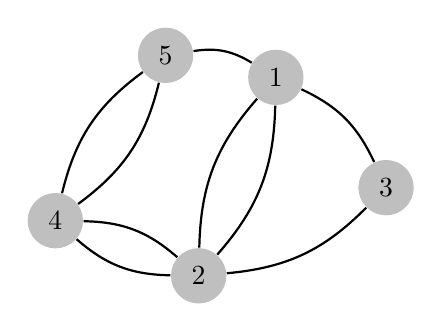
\begin{tikzpicture} [
                scale=1.4,
                vertex/.style={circle,fill=black!25,minimum size=20pt,inner sep=0pt},
                edge/.style = {draw,thick,-},
                selected edge/.style = {draw,line width=5pt,-,red!50},
                bent right/.style = {bend right=20},
                bent left/.style = {bend left=20},
            ]
            % First we draw the vertices
            \foreach \pos/\name/\label in {
                    {(1,2)/a/5},
                    {(2,1.8)/b/1},
                    {(1.3,0)/c/2},
                    {(0,0.5)/d/4},
                    {(3,0.8)/e/3}}
                % \node[vertex] (\name) at \pos {$\name \label$};
                \node[vertex] (\name) at \pos {$\label$};
            % Connect vertices with edges and draw weights
            \foreach \source/ \dest in {
                    a/d,d/a,
                    b/a,
                    b/c,c/b,
                    c/e,
                    c/d,d/c,
                    e/b}
                \path[edge] (\source) edge [bent right] (\dest);
        \end{tikzpicture}
    \end{subfigure}
    \quad
    %%%%%%%%%%%%%%%%%%%%%%%%%%%%%%%%%%%%%%%%%%%%%%%%%%%%%%%%%%%%%%%%%%%%%%%%%%%%%%%%%%%%%
    \begin{subfigure}[b]{0.45\textwidth}
        \centering
        \caption{Grafo dopo la contrazione di $\left\{ 1, 2 \right\}$}
        \label{fig:ex_contrazione:dopo}
        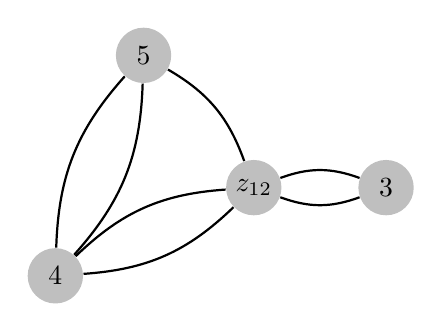
\begin{tikzpicture} [
                scale=1.4,
                vertex/.style={circle,fill=black!25,minimum size=20pt,inner sep=0pt},
                edge/.style = {draw,thick,-},
                selected edge/.style = {draw,line width=5pt,-,red!50},
                bent right/.style = {bend right=20},
                bent left/.style = {bend left=20},
            ]
            % First we draw the vertices
            \foreach \pos/\name/\label in {
                    {(0.8,2)/a/5},
                    {(1.8,0.8)/c/z_{12}},
                    {(0,0)/d/4},
                    {(3,0.8)/e/3}}
                % \node[vertex] (\name) at \pos {$\name \label$};
                \node[vertex] (\name) at \pos {$\label$};
            % Connect vertices with edges and draw weights
            \foreach \source/ \dest in {
                    a/d,d/a,
                    c/a,
                    c/e,
                    c/d,d/c,
                    e/c}
                \path[edge] (\source) edge [bent right] (\dest);
        \end{tikzpicture}
    \end{subfigure}
\end{figure}

\subsubsection{Effetti della contrazione su un taglio}

Ogni taglio $C'$ sul grafo contratto ha un suo corrispettivo nel grafo originale con la stessa taglia.
Questo implica che il taglio minimo in $
\bgg{} / e
$ può solo essere più grande.
Il taglio minimo deve corrispondere ad un taglio con la stessa cardinalità in $\bgg{}$ e quindi il taglio minimo può solo crescere.
\begin{theorem}
    Per ogni 
    % $\forall$
    taglio $C'$ di $
    \bgg{} / e
    = \left\{ u,v \right\}
    $,
    esiste
    % $\exists$
    $C$ taglio di $
    \bgg{}
    $ con $|C|=|C'|$.
\end{theorem}
\begin{proof}
    Sia $
    \bgg{} / e 
    =
    \left( V', E' \right)
    $, e $
    C' \subseteq E'
    $ un taglio, per cui $
    C'
    $ disconnette $
    \bgg{} / e 
    $.
    Si consideri l'insieme di archi $
    C \in E\left( \bgg{} \right)
    $ ottenuto da $C'$ sostituendo ogni archo $
    \left\{ 
        z_{uv}, x
    \right\}
    \in C'
    $ con il corrispettivo arco $
    \left\{ u,x \right\}
    $ o $
    \left\{ v,x \right\}
    $ in $
    E \left( \bgg{} \right)
    $.
    Riguardo alla cardinalità, si sostituisce un arco con un altro, quindi sono uguali.
    Va dimostrato che $C$ è un taglio.
    \\
    Se $C'$ non contiene nessun arco che abbia $
    z_{uv}
    $ come estremo, $C'$ è già un taglio in $
    \bgg{} / e
    $ e disconnette anche $
    \bgg{}
    $.
    \\
    Si sa che $C'$ disconnette $
    \bgg{} / e
    $, e disconnette $
    z_{uv}
    $ da qualche nodo $x$.
    La rimozione del taglio crea almeno due componenti connesse, 
    una componente connessa che contiene $
    z_{uv}
    $ e un'altra componente connessa che contiene $x$.
    Questo significa che ogni cammino da $
    z_{uv}
    $ a $x$ in $
    \bgg{} / e
    $ deve contenere un arco di $C'$.
    \\
    Si supponga che in $
    \bgg{}
    $, $C$ non sia un taglio, ovvero in $
    \bgg{}
    $ sono tutti nella stessa componente connessa, ovvero $C$ non ha disconnesso il grafo.
    Per esempio esiste un cammino tra $u$ e $x$ che usa solo archi in $E - C$, ovvero non usa archi in $C$.
    Se non usa archi in $C$, diventa un cammino tra $
    z_{uv}
    $ e $x$ che non usa archi in $C'$.
    Di conseguenza, si contraddice l'ipotesi che $
    z_{uv}
    $ fosse disconnesso da $x$ in $
    \bgg{} / e
    $ a cui si è rimosso $C'$, perché c'è un cammino tra $
    z_{uv}
    $ e $x$ che non usa archi in $C'$.
\end{proof}
\begin{corollario}
    Vale
    % \begin{equation*}
    $
        |
        \mincut
        \left( 
            \bgg{} / e
        \right)
        |
        \geq
        |
        \mincut
        \left( 
            \bgg{}
        \right)
        |
    % \end{equation*}
    $
    \begin{proof}
        Tutte le cardinalità dei tagli in $
        \bgg{} / e
        $ sono realizzate anche in $
        \bgg{}
        $.
    \end{proof}
\end{corollario}
\begin{corollario}
    Se $C$ è un taglio di $
    \bgg{}
    $ con $
    e \notin C
    $, allora l'insieme $C'$ corrispondente a $C$ in $
    \bgg{} / e
    $ è un taglio in $
    \bgg{} / e
    $.
\end{corollario}
\noindent
Si possono identificare in questo modo i tagli che vengono distrutti.
La contrazione infatti mantiene i tagli che sopravvivono nel grafo $
\bgg{} / e
$ e distrugge gli altri tagli.
Questo caratterizza tutti i tagli che scompaiono, che sono tutti i tagli che contengono $e$.
% TODO grafico due grafi connessi 137.8
Se \emph{non} si contrae rispetto a un arco del taglio minimo, quel taglio sopravvive.
\begin{proof}
    Sia $
    e = \left\{ u,v \right\}
    $, e sia $C$ un taglio che non contiene $e$.
    Nella rimozione di $C$ da $E$, si creano almeno due componenti connesse e
    $u$ e $v$
    devono risultare nella stessa componente connessa: $e$ non è parte del taglio, per cui 
    $u$ e $v$
    devono essere connessi.
    Un cammino tra due nodi in due componenti connesse diverse dovrebbe utilizzare un arco del taglio.
    Considerando $x$ in una componente connessa diversa, si considerano in $
    \bgg{} / e
    $ i nodi $
    z_{uv}
    $ e $x$.
    Il cammino tra $
    z_{uv}
    $ e $x$ era originariamente da 
    $u$ a $x$
    o da
    $v$ a $x$.
    Deve quindi utilizzare un arco del taglio originario (modificato rispetto alla contrazione).
    Perché altrimenti sopravviverebbe in $
    \bgg{} / e
    $ un cammino che non usa nessun arco nel taglio $C'$ corrispettivo a $C$, ma quel cammino esisterebbe anche nel grafo originario, e $C$ non sarebbe un taglio.
\end{proof}
% Un taglio disconnette il grafo in più componenti connesse
% in questo caso se il taglio non contiene questo arco
% u e v devono essere nella stessa componente connessa
% e quindi tutti i cammini verso x useranno sempre almeno un arco di C
% allora questi cammini nel grafo contratto da zuv a x
% devono per forza usare un arco dell'insieme trasformato
% altrimenti quel cammino sopravviverebbe in G contratto rispetto ad e
% e sopravviverebbe anche in questo grafo privato di C.

\subsection{Algoritmo di Karger}
% pag 138.8

\subsubsection{Implementazione}

Si è dimostrato che se si contrae su un arco $e \notin C$, se $C$ era un taglio in $
\bgg{}
$, allora $C'$ è un taglio in $
\bgg{} / e
$.
Rimangono allora tutti e soli i tagli che non contengono $e$.
Gli archi cambiano nomenclatura, ma rimane lo stesso taglio.

L'idea di Karger è sperare di evitare di contrarre su un arco del taglio
% che sarebbe un aglio
minimo, e in questo modo conservare il taglio minimo.
Nel fascio di archi che si restituisce alla fine ci sarà proprio il taglio minimo.

Va studiato con che probabilità si riesce ad evitare di contrarre il taglio minimo.
Questo capita con una probabilità non bassissima:
il taglio è minimo per definizione, e ha taglia molto piccola rispetto al numero totale di archi.
Selezionare un arco di uno specifico taglio minimo avviene allora con probabilità moderata.

\begin{algorithm}[H]
\caption{Full contraction}\label{alg:full_contraction}
\begin{algorithmic}[1]
    \Procedure{Full\_Contraction}{$\bgg{}$}
        \State $n \gets |V \left( \bgg{} \right)|$
        \For{$i \gets 1 $ to $ n - 2 $ }
            \State $e \gets $
            \Call{Random}{$E\left( \bgg{} \right)$}
            \State $\bgg{} \gets \bgg{} / e $
        \EndFor
        \State return $|E\left( \bgg{} \right)|$
    \EndProcedure
\end{algorithmic}
\end{algorithm}
\noindent
L'algoritmo ha complessità lineare nel numero di archi di $
\bgg{}
$: $
T_{FC} \left( n, m \right)
=
\Theta \left( m \right)
$.
\\
La $
\Call{Full\_Contraction}{\bgg{}}
$ genera un qualche taglio (che è anche un node-cut).
L'algoritmo di \emph{Karger} amplifica la probabilità di essere corretto:
si vuole ottenere il taglio minimo, quindi si fa girare più volte la contrazione e si preserva il taglio più piccolo trovato. 
Anche se l'algoritmo non è decisionale, vale l'amplificazione, con la speranza che se il taglio minimo si individua con una certa probabilità, prima o poi lo si individua.

\begin{algorithm}[H]
\caption{Karger}\label{alg:karger}
\begin{algorithmic}[1]
    \Procedure{Karger}{$\bgg{}, k$}
        \State $min \gets |E(\bgg{})| $
        \RepLoop{$k$}
            \State $t \gets \Call{Full\_Contraction}{\bgg{}} $
            \State $min \gets \Call{Min}{min, t} $
        \EndRepLoop
        \State return $min$
    \EndProcedure
\end{algorithmic}
\end{algorithm}
\noindent
Rispetto all'algoritmo deterministico, che deve costruire strutture complesse per sconfiggere il caso peggiore (cammini aumentanti\ldots), l'algoritmo randomizzato supera il caso peggiore con l'idea di schivare alcuni elementi, sfruttando proprio la randomizzazione della scelta.

\subsubsection{Rapido recap di probabilità}

Dati due eventi indipendenti $
E_1
$ e $
E_2
$, la probabilità che avvengano entrambi vale
\begin{equation*}
    \prob{
        E_1 \cap E_2
    }
    =
    \prob{E_1}
    \prob{E_2}
\end{equation*}
Se invece non sono indipendenti, la probabilità che avvenga il secondo dato che il primo si è verificato vale,
per $
\prob{E_1} > 0
$
\begin{equation*}
    \prob{E_2 \mid E_1}
    =
    \frac{
        \prob{ E_1 \cap E_2 }
    }{
        \prob{E_1}
    }
    \quad
    \leftrightarrow
    \quad
    \prob{ E_1 \cap E_2 }
    =
    \prob{E_1}
    \prob{E_2 \mid E_1}
\end{equation*}
Questo si estende per $n$ eventi
\begin{equation*}
    \prob{
        \bigcap_{i=1}^{h} E_i
    }
    =
    \prob{E_1}
    \prod_{i=2}^{h}
    \prob{
        E_i \mid
        E_1 \cap \cdots \cap E_{i-1}
    }
\end{equation*}

\subsubsection{Analisi dell'algoritmo}

Dato un multigrafo $
\bgg{}
=
\left( V, E \right)
$, il grado di ogni nodo è $
d(v) =
|
\ldblbrace
\left\{ 
    v, x
\right\}
\in E
\rdblbrace
|
$.
Togliendo tutti gli archi incidenti su un nodo, si ottiene un edge-cut valido.
Se il taglio minimo è $
C^*
$ di taglia $
|C^*| = t
$, deve allora valere $
d(v) \geq t
$.
Si può allora mostrare che il numero di archi è grande rispetto alla cardinalità del taglio minimo, infatti
\begin{align*}
    |E|
    &= 
    \sum_{v \in V} d(v)
    \bigg/ 2
    \\
    & \geq 
    \sum_{v \in V} t
    \bigg/ 2
    \\
    &= 
    \frac{nt}{2}
\end{align*}
per cui il numero di archi è circa $n$ volte $t$, e il numero di nodi può facilmente essere molto grande.
Si vuole studiare la probabilità che un certo taglio minimo \emph{fissato} sopravviva alla contrazione
\begin{equation*}
    \prob{
        \text{un taglio minimo fissato $C^*$ sopravvive a full contraction}
    }
\end{equation*}
questa probabilità è di sicuro inferiore a quella relativa a un taglio minimo \emph{generico}, di cui si trova così un lower bound.
\\
Seguendo le operazioni dell'algoritmo, si studia per primo l'evento 
\begin{equation*}
    E_1 = 
    \text{la prima contrazione evita }
    C^*
\end{equation*}
Perché questo avvenga, non si devono selezionare archi del taglio, per cui
\begin{align*}
    \prob{E_1}
    &= 
    1 - 
    \frac{|C^*|}{|E|}
    \\
    &
    \geq
    1 - 
    \frac{t}{nt/2}
    \\
    &= 
    1 - 
    \frac{2}{n}
\end{align*}
e questo è un bound in alta probabilità.
Il secondo evento da analizzare è
\begin{equation*}
    E_2 = 
    \text{la seconda contrazione evita }
    C^*
\end{equation*}
ma si deve considerare questo evento condizionato dal successo di $E_1$:
se $
C^*
$ è sopravvissuto, si trova un taglio trasformato (con nomenclatura degli archi diversa) di taglia uguale $
|C^*|
=
|
C^{*'}
|
=
t
$
\begin{align*}
    \prob{
        E_2 \mid E_1
    }
    &= 
    1 -
    \frac{
        C^{*'}
    }{
        |E\left( \bgg{} / e_1 \right)|
    }
    \\
    &
    \geq
    1 - 
    \frac{t}{(n-1)t/2}
    \\
    &= 
    1 - 
    \frac{2}{n-1}
\end{align*}
La probabilità inizia quindi a degradare, la cardinalità del taglio cercato resta costante, mentre il numero di archi tra cui scegliere diminuisce. Al passo generico $i$
\begin{align*}
    \prob{
        E_i \mid
        E_1 \cap \cdots \cap E_{i-1}
    }
    &
    \geq
    1 - 
    \frac{t}{(n-i+1)t/2}
    \\
    &= 
    1 - 
    \frac{2}{n-i+1}
\end{align*}
Se in tutte le $n-2$ iterazioni il taglio minimo viene evitato, l'algoritmo ritorna il taglio corretto.
\begin{align*}
    \prob{
        \,
        \bigcap_{i=1}^{n-2} E_i
    }
    &= 
    \prod_{i=1}^{n-2}
    \left( 
        1 - 
        \frac{2}{n-i+1}
    \right)
    \\
    &= 
    \prod_{i=1}^{n-2}
    \;
    \frac{
        n-i-1
    }{
        n-i+1
    }
    \\
    &= 
    \frac{
        \cancel{
            n-2
        }
    }{
        n
    }
    \frac{
        \cancel{
            n-3
        }
    }{
        n-1
    }
    \frac{
        \cancel{
            n-4
        }
    }{
        \cancel{
            n-2
        }
    }
    \ldots
    \frac{
        \cancel{
            3
        }
    }{
        \cancel{
            5
        }
    }
    \frac{
        2
    }{
        \cancel{
            4
        }
    }
    \frac{
        1
    }{
        \cancel{
            3
        }
    }
    \\
    &= 
    \frac{2}{n(n-1)}
\end{align*}
La probabilità che un taglio minimo sopravviva è quindi molto bassa, ma non trascurabile.
Ripetendo $k$ volte la contrazione
\begin{equation*}
    k = d \frac{n^2}{2} \ln n
\end{equation*}
si riesce ad amplificare la probabilità, sfruttando il fatto che le esecuzioni della contrazione sono indipendenti
\begin{align*}
    \prob{
        \text{$k$ full contraction falliscono}
    }
    &
    \leq
    \left( 
        1 -
        \frac{2}{n(n-1)}
    \right)^k
    \\
    &
    \leq
    \left( 
        1 -
        \frac{2}{n^2}
    \right)^k
    \\
    &
    \leq
    \left( 
        \left( 
            1 -
            \frac{2}{n^2}
        \right)^{n^2/2}
    \right)^{\ln n^d}
    \\
    &
    <
    \left( e^{-1} \right)^{\ln n^d}
    \\
    &= 
    \frac{1}{n^d}
\end{align*}
La complessità è molto elevata: una singola contrazione è lineare nel numero di archi, e viene ripetuta $k$ volte, per cui
\begin{equation*}
    T_{Karger} (n) =
    \Theta \left( 
        m \cdot n^2 \log n
    \right)
\end{equation*}
che per grafi densi risulta quartica in $n$.

\subsection{Variante Karger-Stein}
% pag 141.5

\subsubsection{Implementazione}

Nel corso dell'algoritmo di \emph{Karger}, c'è una progressiva degradazione della probabilità di evitare il taglio minimo cercato: nelle prime iterazioni, ci sono tantissimi archi tra cui scegliere, mentre nelle ultime parecchi archi rimasti sono parte del taglio minimo.
\begin{equation*}
    \text{Prob di successo:}
    \quad
    1 - \frac{2}{n}
    ,
    \;
    1 - \frac{2}{n-1}
    ,
    \;
    1 - \frac{2}{n-2}
    \quad
    \cdots
    \quad
    1 - \frac{2}{4}
    ,
    \;
    1 - \frac{2}{3}
\end{equation*}
In questo modo si stanno sfruttando male le prime contrazioni, che hanno qualità migliore delle finali.
L'idea di \emph{Stein} è proprio quella di fermare la contrazione dopo $k$ iterazioni
andando a riutilizzare i grafi ottenuti all'inizio più volte.
Si arresta quindi la routine $
\Call{Full\_Contraction}{\bgg{}}
$ dopo $k$ contrazioni, e si utilizza il grafo generato per avviare più ricerche indipendenti.
Il processo si ripete ricorsivamente, utilizzando in questo modo i grafi iniziali, di qualità migliore, un numero esponenziale di volte.
I primi due livelli dell'albero generato sono mostrati in \rfig{fig:contrazione_stein}.
\begin{figure}[h]
    \centering
    \caption{Prime due iterazioni dell'algoritmo di \emph{Stein}}
    \label{fig:contrazione_stein}
    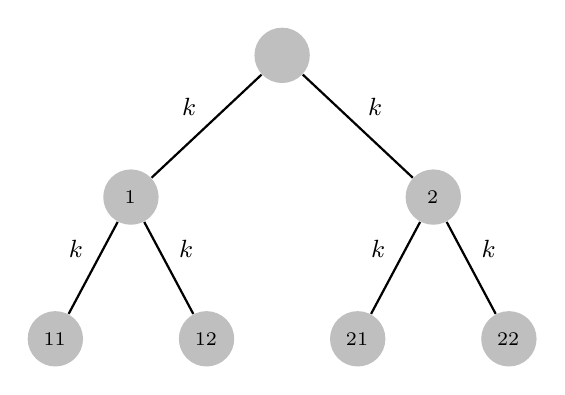
\begin{tikzpicture} [
            auto,
            scale=1.2,
            vertex/.style={circle,fill=black!25,minimum size=20pt,inner sep=0pt},
            edge/.style = {draw,thick,-},
            weight/.style = {font=\small},
        ]
        \foreach \pos/\name/\labin in {
                {(0.8,1.5)/b/\bgg{}_{1}},
                {(0,0)/c/\bgg{}_{11}},
                {(1.6,0)/d/\bgg{}_{12}},
                {(4.0,1.5)/e/\bgg{}_{2}},
                {(3.2,0)/f/\bgg{}_{21}},
                {(4.8,0)/g/\bgg{}_{22}},
                {(2.4,3)/a/\bgg{}}}
            % \node[vertex] (\name) at \pos {$\name \labin$};
            \node[vertex] (\name) at \pos {$\labin$};
        \foreach \source/ \dest in {
                c/b,b/d,b/a,a/e,f/e,e/g}
            \path[edge] (\source) -- node[weight] {$k$} (\dest);
    \end{tikzpicture}
\end{figure}
% L'algoritmo di \emph{Karger-Stein} risulta allora
\begin{algorithm}[H]
\caption{Algoritmo di \emph{Karger-Stein}}\label{alg:karger_stein}
\begin{algorithmic}[1]
    \Procedure{R\_KS}{$\bgg{}$}
        \If{$|V(\bgg{})| \leq 8$}
            \State * ritorna il \emph{min-cut} calcolato con algoritmo deterministico *
        \EndIf
        \State $k \gets 
        % f (V(\bgg{}))$ 
        n -
        \left\lceil 
            \frac{n}{\sqrt{2}} + 1
        \right\rceil
        $ 
        \State $\bgg{}_{1} \gets \Call{Partial\_Contraction}{\bgg{}, k} $
        \State $t_{1} \gets \Call{R\_KS}{\bgg{}_{1}} $
        \State $\bgg{}_{2} \gets \Call{Partial\_Contraction}{\bgg{}, k} $
        \State $t_{2} \gets \Call{R\_KS}{\bgg{}_{2}} $
        \State return $\Call{Min}{t_1, t_2} $
    \EndProcedure
\end{algorithmic}
\end{algorithm}
\noindent
% Nella contrazione parziale vengono eseguite molte iterazioni, ma meno delle $n-2$ della contrazione totale.
Il costo per calcolare il $
\mincut
$ su grafi di taglia piccola è costante.
Ad ogni iterazione,
vengono effettuate due chiamate ricorsive, ciascuna invocata sui grafi generati, di taglia
\begin{equation*}
    |
    V(\bgg{}_{1})
    | = |
    V(\bgg{}_{2})
    | = 
    n - k = 
    \left\lceil 
        \frac{n}{\sqrt{2}} + 1
    \right\rceil
\end{equation*}
Il costo di una contrazione parziale è $
O \left( n^2 \right)
$.
% (tenere traccia del numero esatto di archi è troppo complicato).
La complessità dell'algoritmo si può quindi determinare
risolvendo l'equazione di ricorrenza
\begin{equation*}
    T(n) =
    \begin{cases}
        c & n \leq 8
        \\
        2
        T\left( 
            \left\lceil 
                \frac{n}{\sqrt{2}} + 1
            \right\rceil
        \right)
        +
        O \left( n^2 \right)
        &
        n > 8
    \end{cases}
\end{equation*}
La funzione si semplifica in 
\begin{equation*}
    T(n) =
    2
    T\left( 
        \frac{n}{\sqrt{2}}
    \right)
    +
    O \left( n^2 \right)
\end{equation*}
Applicando il \emph{master theorem}, il work per iterazione è $
O \left( n^2 \right)
$, mentre la funzione di soglia risulta $
n^{\log_{\sqrt{2}} 2} = n^2
$. Le due corrispondono, per cui 
\begin{equation*}
    T(n) = O \left( n^2 \log n \right)
\end{equation*}

\subsubsection{Analisi dell'algoritmo}

Prima di poter studiare la probabilità che l'algoritmo sia corretto, si studia la probabilità che la contrazione parziale mantenga il taglio minimo.
Si consideri il grafo $
\bgg{}
$, di taglia $n$
\begin{align*}
    \prob{
        \text{successo di $
            \Call{PC}{\bgg{}, k}
        $}
    }
    &= 
    \prob{
        \text{$C^*$ sopravvive a $k$ iterazioni}
    }
    \\
    &= 
    \prod_{i=1}^{k}
    \;
    \frac{
        n-i-1
    }{
        n-i+1
    }
    \\
    &= 
    \frac{
        \left\lceil 
            \frac{n}{\sqrt{2}} + 1
        \right\rceil
        \left( 
            \left\lceil 
                \frac{n}{\sqrt{2}} + 1
            \right\rceil
            - 1
        \right)
    }{
        n \left( n-1 \right)
    }
    \intertext{entrambi i fattori al numeratore sono maggiori di $
        n / \sqrt{2}
    $}
    &
    \geq
    \frac{
        \frac{n}{\sqrt{2}}
        \frac{n}{\sqrt{2}}
    }{
        n \left( n-1 \right)
    }
    \\
    &
    \geq
    \frac{1}{2}
\end{align*}
Questa analisi giustifica la scelta di $k$ effettuata: la contrazione parziale ha una probabilità molto più alta di evitare il cammino minimo rispetto alla contrazione totale.
La probabilità di successo di \emph{Karger-Stein} risulta allora
\begin{align*}
    P(n)
    &= 
    \prob{
        \text{successo per $
            |V(\bgg{})|=n
        $}
    }
    \\
    &= 
    1 - 
    \prob{
        \text{fallimento per $
            |V(\bgg{})|=n
        $}
    }
    \\
    &= 
    1 - 
    \prob{
        \text{falliscono entrambe le computazioni, su $
            \bgg{}_{1}
            $ e $
            \bgg{}_{2}
        $}
    }
    \intertext{le due ramificazioni dell'algoritmo sono indipendenti, e ciascuna è formata da una contrazione parziale e una chiamata ricorsiva}
    &= 
    1 - 
    \left[ 
    \vphantom{\big(}
        \prob{
            \text{fallisce la computazione su un ramo fissato}
        }
    \right]^2
    \\
    &= 
    1 - 
    \left[ 
    \vphantom{\big(}
        1 -
        \prob{
            \text{ha successo la computazione su un ramo fissato}
        }
    \right]^2
    \intertext{perché un ramo abbia successo, il cammino minimo deve essere mantenuto dalla contrazione parziale e deve essere restituito correttamente dalla chiamata ricorsiva}
    &= 
    1 - 
    \left[ 
        1 -
        \prob{
            \vphantom{\big(}
            \text{successo di $
                \Call{PC}{\bgg{}, k}
            $}
        }
        \cdot
        \prob{
            \vphantom{\big(}
            \text{successo di $
                \Call{R\_KS}{\bgg{}_1}
            $}
        }
    \right]^2
    \intertext{la probabilità di successo della contrazione è stata calcolata prima e ne si considera il caso peggiore, e per la chiamata ricorsiva si può esprimere il valore in funzione dell'istanza ridotta}
    &
    =
    1 - 
    \left[ 
        1 -
        \frac{1}{2}
        \cdot
        P\left( n - k \right)
    \right]^2
    \\
    &
    =
    1 - 
    \left[ 
        1 -
        \frac{1}{2}
        \cdot
        P\left( 
            \left\lceil 
                \frac{n}{\sqrt{2}} + 1
            \right\rceil
        \right)
    \right]^2
\end{align*}
La probabilità di correttezza del caso base è 1, perché si applica un algoritmo deterministico, per cui la probabilità di successo per un'istanza di taglia $n$ vale
\begin{equation*}
    P(n) =
    \begin{cases}
        1 & n \leq 8
        \\
        1 - 
        \left[ 
            1 -
            \frac{1}{2}
            \cdot
            P\left( 
                \left\lceil 
                    \frac{n}{\sqrt{2}} + 1
                \right\rceil
            \right)
        \right]^2
        &
        n > 8
    \end{cases}
\end{equation*}
Per risolvere questa ricorrenza, si inizia studiando il suo albero delle ricorsioni, di cui si rappresenta un generico cammino radice-foglia in \rfig{fig:albero_prob_stein} (tutti i cammini hanno la stessa altezza)
\begin{figure}[h]
    \centering
    \caption{Uno dei cammini seguiti da \emph{Karger-Stein}}
    \label{fig:albero_prob_stein}
    \begin{tikzpicture} [
            scale=1.2,
            nodo/.style={ellipse,fill=black!25,minimum size=20pt,inner sep=0pt},
            arco/.style = {draw,thin,-},
            arco tratteggiato/.style = {draw,thin,dotted},
        ]
        \foreach \pos/\name/\labin/\labout in {
                {(0,5)/a/n/0},
                {(0,4)/b/
                \left\lceil 
                    \frac{n}{\sqrt{2}} + 1
                \right\rceil
                /1},
                {(0,2.8)/c/S_{i}/i},
                % {(0,2)/d/S_{\bar{i}}/\bar{i}},
            {(0,1.6)/e/<8/\bar{i}}}
            \node[nodo, label={east:$\labout$}] (\name) at \pos {$\labin$};
            % \node[nodo, label={east:$\labout$}] (\name) at \pos {\name $\labin$};
        \foreach \source/ \dest in {
                % d/e,
                a/b}
            \path[arco] (\source) -- (\dest);
        \foreach \source/ \dest in {
                % c/d,
                c/e,
                b/c}
            \path[arco tratteggiato] (\source) -- (\dest);
        \begin{pgfonlayer}{background}
        \end{pgfonlayer}
    \end{tikzpicture}
\end{figure}
\\
La taglia $
S_i
$ del grafo all'iterazione $i$ è limitata da 
\begin{equation*}
    S_i
    \leq
    \left\lceil 
        \frac{
            n
        }{
            \left( 
                \sqrt{2}
            \right)^i
        }
        + 7
    \right\rceil
\end{equation*}
questo si prova per induzione per ESERCIZIO, la base per $i=0$ è chiaramente verificata $n \leq n + 7$, e poi si prova per $i$ dato che vale per $i-1$.
\\
Al livello $
\bar{i}
=
2 \log_2 n
$ la taglia risulta
\begin{align*}
    S_{\bar{i}}
    &
    \leq
    \left\lceil 
        \frac{
            n
        }{
            \left( 
                \sqrt{2}
            \right)^{\bar{i}}
        }
        + 7
    \right\rceil
    \\
    &=
    \left\lceil 
        \frac{
            n
        }{
            \left( 
                \sqrt{2}
            \right)^{
                2 \log_2 n
            }
        }
        + 7
    \right\rceil
    \\
    &=
    \left\lceil 
        \frac{
            n
        }{
            n
        }
        + 7
    \right\rceil
    \\
    &= 
    8
\end{align*}
Per cui al livello $
\bar{i}
$ si raggiunge la foglia.
Se $h$ è il livello preso in considerazione nell'albero, sarà limitato da
\begin{equation*}
    h \leq 1 +
    \left\lceil 
        2 \log_2 n
    \right\rceil
\end{equation*}
La funzione di ricorrenza si può riscrivere in funzione del livello $h$ in cui si è dell'albero
\begin{equation*}
    P(h) =
    \begin{cases}
        1 & h = 1
        \\
        1 - 
        \left[ 
            1 -
            \frac{1}{2}
            \cdot
            P\left( 
                h - 1
            \right)
        \right]^2
        &
        h > 1
    \end{cases}
\end{equation*}
Si dimostra per induzione che
\begin{equation*}
    P(h) \geq
    \frac{1}{h}
\end{equation*}
La base per $h=1$ è chiaramente vera.
Supponendo che sia vero per $h-1$, lo si dimostra per $h$.
Esplicitando il quadrato per $h>1$ vale
\begin{equation*}
    P(h) =
    P(h-1)
    -
    \frac{1}{4}
    \left( 
        P
        (h-1)
    \right)
    ^2
\end{equation*}
Si consideri la funzione reale, definita $\forall x$
\begin{equation*}
    f(x) = x - \frac{1}{4} x^2
\end{equation*}
Questa funzione, calcolata nel punto $
    P(h-1)
$, vale proprio $
    P(h)
$:
\begin{equation*}
    f(
        P(h-1)
    ) = 
    P(h)
\end{equation*}
e nell'intervallo $x \in [0,1]$ ha derivata positiva, ed è quindi una funzione crescente.
Per l'ipotesi induttiva vale
\begin{align*}
    P(h-1)
    &
    \geq
    \frac{1}{h-1}
    \intertext{e il verso della disequazione viene mantenuto dall'applicazione di una funzione crescente}
    f(
        P(h-1)
    )
    &
    \geq
    f\left( 
        \frac{1}{h-1}
    \right)
    \intertext{sostituendo il primo membro e espandendo il secondo}
    P(h)
    &
    \geq
    \frac{1}{
        h-1
    }
    -
    \frac{1}{
        4
        \left( 
            h-1
        \right)^2
    }
    \\
    &
    >
    \frac{1}{
        h-1
    }
    -
    \frac{1}{
        2
        \left( 
            h-1
        \right)^2
    }
    \\
    &
    =
    \frac{1}{
        h-1
    }
    -
    \frac{1}{
        2
        \left( 
            h-1
        \right)
        \left( 
            h-1
        \right)
    }
    \intertext{per $h \geq 2$ vale $2(h-1) \geq h$}
    &
    \geq
    \frac{1}{
        h-1
    }
    -
    \frac{1}{
        h
        \left( 
            h-1
        \right)
    }
    \\
    &= \frac{1}{h}
    \intertext{si era mostrato che $
        h \leq 1 +
        \left\lceil 
            2 \log_2 n
        \right\rceil
    $}
    \\
    &
    \geq
    \frac{1}{
        \left\lceil 
            2 \log_2 n
        \right\rceil
        + 1
    }
    \\
    &
    \geq
    \frac{1}{
        4 \log_2 n
    }
\end{align*}
Quindi la probabilità di successo è legata all'inverso del logaritmo, invece che all'inverso del quadrato come per l'algoritmo di \emph{Karger}.
Sono quindi necessarie meno iterazioni per ottenere la correttezza in alta probabilità.
Ripetendo l'algoritmo di \emph{Karger-Stein} per
\begin{equation*}
    s
    =
    d
    \,
    4 \log_2 n
    \,
    \ln n
\end{equation*}
volte, l'algoritmo fallisce se tutte le esecuzioni sbagliano, ovvero
\begin{align*}
    \prob{
        \text{insuccesso dopo $s$ iterazioni}
    }
    &
    \leq
    \left[ 
        1 -
        \frac{1}{
            4 \log_2 n
        }
    \right]^{
        d
        \,
        4 \log_2 n
        \,
        \ln n
    }
    \\
    &
    <
    \left( e^{-1} \right)^{
        \ln n
        ^{
            d
        }
    }
    \\
    &
    \leq
    \frac{1}{
        n^d
    }
\end{align*}


\section{Esempi di algoritmi randomizzati}

\subsection{Polling}

Si vuole stimare in maniera randomizzata una certa quantità.
Utilizzando un metodo detto stima di Montecarlo, per cui si ricavano stime di quantità con esperimenti randomizzati.

Si consideri un'urna $U$ contenente $n$ palline, nel caso più semplice di due colori, bianco e nero.
Si vuole stimare 
\emph{esattamente} 
la proporzione $\alpha$ di palline bianche.
L'urna contiene quindi $
\alpha n
$ palline bianche e $
(1-\alpha) n
$ palline nere.

È necessario conoscere un limite inferiore deterministico alla quantità di palline bianche, per cui
\begin{equation*}
    \prob{
        \alpha \geq \alpha_{min}
    } 
    = 1
\end{equation*}
Questo perché se le palline bianche sono eccessivamente rare, non c'è verso di stimarne la frequenza.
Si vuole ottenere una stima randomizzata $
\bm{\beta}
$ di $\alpha$, con la garanzia che la stima sia 
con confidenza $
0 < \delta < 1
$
all'interno di una certa precisione fissata $
0 < \varepsilon < 1
$, ovvero l'errore relativo è limitato da
\begin{equation*}
    \prob{
        \frac{
            |
            \bm{\beta}
            - \alpha
            |
        }{
            \alpha
        }
        > \varepsilon
    }
    < \delta
\end{equation*}
\begin{algorithm}[H]
\caption{Polling}\label{alg:polling}
\begin{algorithmic}[1]
    \Procedure{Approximate\_$\alpha$}{$U, \varepsilon, \delta, \alpha_{min}$}
        \State $n \gets U$
        \State $x \gets 0$
        \State $k \gets f \left( n, \varepsilon, \delta, \alpha_{min} \right)$
        \RepLoop{$k$}
            \State $p \gets
            \Call{Random}{U}
            $
        \EndRepLoop
        \If{$p.color = $ \texttt{bianco}}
            \State $x \gets x + 1$
        \EndIf
        \State return $\beta = x / k$
    \EndProcedure
\end{algorithmic}
\end{algorithm}
\noindent
Nota: le estrazioni sono \emph{con} reimbussolamento.
Si associa una variabile indicatrice a ciascuna estrazione, ottenendo $k$ variabili i.i.d. 
\begin{equation*}
    X_i =
    \begin{cases}
        1 & p.color = B
        \\
        0 & \text{altrimenti}
    \end{cases}
\end{equation*}
Per cui vale chiaramente $
\prob{X_i = 1} = \alpha
$ e
\begin{equation*}
    X = \sum_{i=1}^{k} X_i
    \quad
    \E{X} = \mu = k \alpha
\end{equation*}
E si riscrive l'evento associato ad un eccessivo errore relativo come
\begin{align*}
    \frac{
        |
        \bm{\beta}
        - \alpha
        |
    }{
        \alpha
    }
    &
    > \varepsilon
    \\
    \frac{
        |
        x/k 
        - \alpha
        |
    }{
        \alpha
    }
    &
    > \varepsilon
    \\
    \frac{
        |
        x
        - k \alpha
        |
    }{
        k \alpha
    }
    &
    > \varepsilon
    \\
    \frac{
        |
        x
        - \mu
        |
    }{
        \mu
    }
    &
    > \varepsilon
    \intertext{che equivale alla disgiunzione degli eventi}
    x > (1 + \varepsilon) \mu
    \quad
    &
    \cup
    \quad
    x < (1 - \varepsilon) \mu
    \intertext{e quindi è l'unione di due eventi che si possono limitare con Chernoff}
    \prob{
        \frac{
            |
            x
            - \mu
            |
        }{
            \mu
        }
        > \varepsilon
    }
    &
    <
    e^{- \varepsilon^2 \mu / 2}
    +
    e^{- \varepsilon^2 \mu / 3}
    \\
    &
    <
    2
    e^{- \varepsilon^2 \mu / 3}
    \\
    &
    =
    2
    e^{- \varepsilon^2 k \alpha / 3}
    \\
    &
    \leq
    2
    e^{- \varepsilon^2 k \alpha_{min} / 3}
    \\
    &
    \meq
    \delta
    \intertext{da cui si ricava il valore di $k$ per rispettare $\delta$:}
    k &= 
    \frac{3}{
        \alpha_{min}
        \varepsilon^2
    }
    \ln \left( \frac{2}{\delta} \right)
\end{align*}
Per cui è presente un forte dipendenza dalla precisione $\varepsilon$, mentre la dipendenza rispetto alla confidenza $\delta$ è più blanda.
Per il caso con palline di più colori, si sfrutta l'union bound per ampliare l'analisi.

\subsection{Enumerazione randomizzata (coupon collecting)}

Dato $
\Call{Random}{\left\{ 1, n \right\}}
$ si vuole calcolare il numero medio di invocazioni del metodo necessarie ad estrarre (con molteplicità) tutti i valori in $
\left\{ 1, 2, \cdots, n \right\}
$.
Si vuole calcolare quante estrazioni (\emph{con} reimbussolamento) sono necessarie per essere sicuri di aver visto tutti gli elementi nell'urna.

Spesso ci sono processi in cui l'urna rappresenta un insieme di job, ma non si possono assegnare i lavori agli esecutori in maniera deterministica.
Se un esecutore si guastasse, alcuni job non sarebbero eseguiti.
Assegnando i job casualmente, con un numero limitato di estrazioni tutti i job sono correttamente assegnati.

Sia $
Y \sim Geom (p)
$ una variabile geometrica,
valgono
\begin{equation*}
    \prob{Y = j} = \left( 1-p \right)^{j-1} p
    \qquad
    \E{Y} = \frac{1}{p}
\end{equation*}

Si consideri $
Z_i
$ il numero di chiamate necessarie ad ottenere l'$i$-esimo valore distinto dopo averne visti $
i-1
$, con $
1 \leq i \leq n
$: $
Z_i \sim Geom (p_i)
$
Le prime estrazioni avranno spesso successo, mentre quando quasi tutti gli elementi sono già stati visti, è più raro trovarne uno nuovo.
La variabile viene rappresentata da $p_i$, ottenuto come il numero di valori ancora da vedere diviso il numero totale.
\begin{equation*}
    p_i = 
    \frac{n - \left( i-1 \right)}{n}
    \qquad
    \E{Z_i}
    = 
    \frac{1}{p_i}
    =
    \frac{n}{n-i+1}
\end{equation*}
Il numero complessivo di lanci (che non è una geometrica)
\begin{equation*}
    Z =
    \sum_{i=1}^{n} Z_i
\end{equation*}
allora la media vale
\begin{align*}
    \E{Z}
    &= 
    \sum_{i=1}^{n}
    \E{ Z_i }
    \\
    &= 
    \sum_{i=1}^{n}
    \frac{n}{n-i+1}
    \\
    &= 
    n
    \sum_{i=1}^{n}
    \frac{1}{n-i+1}
    \intertext{effettuando il cambio di variabile $j = n-i+1$}
    &= 
    n
    \sum_{i=1}^{n}
    \frac{1}{j}
    \intertext{la sommatoria è l'$n$-esimo numero armonico}
    &= 
    n H(n)
    \intertext{l'$n$-esimo numero armonico si approssima con il logaritmo}
    &= 
    n \left( \ln n + O (1) \right)
    \\
    &= 
    n \ln n + O(n)
\end{align*}
Ogni job viene quindi assegnato $\log n$ volte, che non è troppo.

Per quanto riguarda la concentrazione intorno alla media, fissato $
i \in \left\{ 1, \cdots, n \right\}
$, la probabilità di non aver collezionato $i$ dopo $r$ lanci ($r>0$) 
corrisponde all'estrazione di un altro valore in tutti i lanci
% data dal $
% (n-1)/n
% $
\begin{equation*}
    \prob{
        E_i^r
    }
    =
    \left( \frac{n-1}{n} \right)^{r}
    =
    \left( 1- \frac{1}{n} \right)^{n \cdot
        r/n
        % \frac{r}{n}
    }
    <
    e^{-r/n}
\end{equation*}
si può scegliere $r$ in modo da limitare questo valore in maniera arbitraria
\begin{align*}
    e^{-r/n}
    &= 
    \frac{1}{n^2}
    \\
    \Rightarrow
    r &= 
    2 n \ln n 
\end{align*}
in generale, la probabilità che dopo $r$ lanci almeno un elemento generico non sia ancora uscito è pari a 
\begin{align*}
    \prob{
        \bigcup_{i=1}^{n}
        E_i^r
    }
    &
    \leq
    \sum_{i=1}^{n}
    \prob{
        E_i^r
    }
    \leq
    n \frac{1}{n^2}
    =
    \frac{1}{n}
\end{align*}
per cui la probabilità che dopo $
2 n \ln n 
$ passi un elemento non sia ancora stato estratto è bassa, minore di $
1/n
$ e la probabilità complementare risulta
\begin{align*}
    \prob{
        \text{tutti estratti in un numero $
            2 n \ln n 
        $ estrazioni}
    }
    \geq 1 - \frac{1}{n}
\end{align*}

Il numero di iterazioni necessarie non è facilmente abbassabile, la probabilità che tutti gli elementi vengano estratti prima della media è minore di $
e^{-c}
$

\subsection{Generazione di bit senza bias}

Si vuole generare un bit che assuma valore 0 o 1 con uguale probabilità, avendo a disposizione un generatore con bias $p$ non noto.

\begin{align*}
    b =
    \begin{cases}
        0 & 
        \text{con prob. }
        1/2
        \\
        1 & 
        \text{con prob. }
        1/2
    \end{cases}
    \qquad
    \Call{Bias}{ }
    =
    \begin{cases}
        0 & 
        \text{con prob. }
        p
        \\
        1 & 
        \text{con prob. }
        1-p
    \end{cases}
\end{align*}
Avendo a disposizione solo la primitiva $
\Call{Bias}{ }
$ si possono estrarre numeri senza bias:
\begin{algorithm}[H]
\caption{Estrazione di bit senza bias}\label{alg:unbias}
\begin{algorithmic}[1]
    \Procedure{Unbias}{ }
        \Repeat
            \State $x \gets
            \Call{Bias}{ }
            $
            \State $y \gets
            \Call{Bias}{ }
            $
        \Until{$x \ne y$}
        \State return $x$
    \EndProcedure
\end{algorithmic}
\end{algorithm}
\noindent
Ad ogni round vengono quindi estratti due valori, e si considera un successo il caso in cui sono valori diversi. Le probabilità delle quattro combinazioni di valori risultano
\begin{equation*}
    \begin{array}[h]{cc|c}
        x & y & \text{prob} \\
        \hline
        \rule{0pt}{1.0\normalbaselineskip}
        0 & 0 & (1-p)^2 \\
        0 & 1 & p(1-p) \\
        1 & 0 & p(1-p) \\
        1 & 1 & p^2
    \end{array}
\end{equation*}
In questo modo vengono individuati due eventi equiprobabili, indipendenti dal bias, che si riesce a distinguere.
L'algoritmo è corretto perché restituisce un bit, e termina per $0<p<1$, anche se prevede in generale computazioni di lunghezza illimitata.
\\
Considerando gli eventi
\begin{equation*}
    A_i = \text{``$
    \Call{Unbias}{ }
    $ termina al round $i$''}
\end{equation*}
che sono indipendenti, dato che o termina al round $i$ o al round $j$, e vale
\begin{equation*}
    \prob{
        \bigcup_{i=1}^{\infty} A_i
    }
    = 1
\end{equation*}
perché prima o poi termina.
Usando la probabilità totale, si riscrive
\begin{align*}
    \prob{
        \Call{Unbias}{ }
        = 1
    }
    &= 
    \sum_{i=1}^{\infty}
    \prob{
        \Call{Unbias}{ }
        = 1
        \mid
        A_i
    }
    \prob{
        A_i
    }
    \intertext{l'algoritmo termina quando capita uno di due eventi equiprobabili}
    &= 
    \sum_{i=1}^{\infty}
    \frac{1}{2}
    \prob{
        A_i
    }
    \\
    &= 
    \frac{1}{2}
    \sum_{i=1}^{\infty}
    \prob{
        A_i
    }
    \intertext{gli eventi $A_i$ sono disgiunti}
    &= 
    \frac{1}{2}
\end{align*}
Per quanto riguarda il numero di round, è descritto da una geometrica con probabilità di successo $
q = 2 p (1-p)
$
\begin{equation*}
    \text{\# round}
    \sim Geom\left( 
        2 p (1-p)
    \right)
    \qquad
    \E{
        \text{\# round}
    }
    =
    \frac{1}{
        2 p (1-p)
    }
\end{equation*}


\subsection{Approssimazione randomizzata}

\section{Pezzi utili di \LaTeX{}}

\subsection{Template vari}

\begin{algorithm}[H]
\caption{Divide and Conquer}\label{alg:dnc}
\begin{algorithmic}[1]
    \Procedure{Divide\&Conquer}{$i$}
        \If{$|i| \leq n_0$}
        \Comment{BASE}
            \State *risolvo direttamente*
        \EndIf
        \State $\langle i_1, i_2, \dots, i_k \rangle \gets A_D(i)$ 
        \Comment{DIVIDE}
        \For{$j \gets 1 $ to $ k $ }
        \Comment{RECURSE}
            \State $s_j \gets
            \Call{Divide\&Conquer}{i_j}
            $
        \EndFor
        \State $s \gets A_C(\langle s_1, s_2, \dots, s_k \rangle)$
        \Comment{CONQUER}
        \State return $s$
    \EndProcedure
\end{algorithmic}
\end{algorithm}
\noindent
Testo non identato!
\begin{algorithm}[H]
\caption{Esempi in libertà}\label{alg:esempi}
\begin{algorithmic}[1]
    \Procedure{Esempi}{$n$}
        \If{$|i| \leq n_0$}
        \Comment{if}
            \State *risolvo direttamente*
        \EndIf
        \ForAll{$i \in A_n$}
        \Comment{for each}
            \State $s \gets
            \Call{Magic}{i}
            $
        \EndFor
        \RepLoop{$k$}
        \Comment{repeat some times}
            \State $t \gets \Call{Full\_Contraction}{\bgg{}} $
            \State $min \gets \Call{Min}{min, t} $
        \EndRepLoop
        \State \Return $x$
        \Comment{il return che vorrei}
    \EndProcedure
    \Function{Unbias}{ }
        \Comment{funzioni}
        \State \Return $0$
    \EndFunction
\end{algorithmic}
\end{algorithm}

\begin{definition}[Algoritmo]\label{def:algex}
    Un algoritmo è una procedura computazionale finita (terminante) e deterministica, specificata come una sequenza di passi elementari (istruzioni) estratte da un insieme standard associato a un modello computazionale (astrazione di un computer) che trasforma in maniera univoca un ingresso in un uscita.
\end{definition}

Guarda che so fare
\begin{align*}
    &
    \setzo{m}
    \quad
    \setzo{}
    \quad
    \odot
    \quad
    \oplus
    \quad
    \zz{n}
    \quad
    \zs
    \quad
    \zs{\rho(n)}
    \quad
    \equiv_n
    \\
    &
    \ldblbrace
        u = 1
    \rdblbrace
    \ldblbraceb
        u = 1
    \rdblbraceb
    \ldblbraceB
        u = 1
    \rdblbraceB
    \ldblbracebb
        u = 1
    \rdblbracebb
    \ldblbraceBB
        u = 1
    \rdblbraceBB
    \\
    &
    \ldblbrace
        \left\{ x, y \right\}
        :
        \left( x = u \right)
        \vee
        \left( y = v \right)
    \rdblbrace
\end{align*}

Un problema
\begin{align*}
    SS: & \\
    \texttt{istanza:} \quad &
    \langle
        S,t
    \rangle
    \\
    \text{dove} \quad &
    S \subseteq \mathbb{N} - \left\{ 0 \right\} \text{ finito}
    \\
    &
    t \subseteq \mathbb{N} - \left\{ 0 \right\} \\
    \texttt{domanda:} \quad &
    \exists \, S' \subseteq S : \sum_{s \in S'}^{} s = t \, ?
\end{align*}

Una lista
\begin{itemize}[noitemsep,parsep=0pt,partopsep=0pt,topsep=0pt]
    \item[--] $L_A = L$ (il linguaggio deciso da $A$ è $L$)
    \item[--] $T_A(|x|) = O(|x|^k)$ per qualche costante $k \geq 0$
\end{itemize}

Una tabella con spazi aggiunti \url{https://tex.stackexchange.com/a/65128}
\begin{equation*}
    \begin{array}[h]{cc|c}
        x & y & \text{prob} \\
        \hline
        \rule{0pt}{1.0\normalbaselineskip}
        0 & 0 & (1-p)^2 \\
        0 & 1 & p(1-p) \\
        1 & 0 & p(1-p) \\
        1 & 1 & p^2
    \end{array}
\end{equation*}

\subsection{Teoremi e vari ambienti }

\begin{theorem}
    Un teorema senza nome
\end{theorem}

\begin{corollario}
    Un primo corollario
\end{corollario}

\begin{corollario}
    Un secondo corollario
\end{corollario}

\begin{theorem}[Nome del teorema]
    Un teorema con nome
\end{theorem}

\begin{corollario}
    Un primo corollario del teorema con nome
\end{corollario}

\begin{definition}
    Una definizione utile, la seconda di questa sezione
\end{definition}

\begin{proposizione}[Nome della proposizione]
    Una proposizione con nome
\end{proposizione}

\begin{corollario}
    Un primo corollario della proposizione con nome
\end{corollario}

\subsection{Grafi}

Grafi facili da mantenere

% Declare layers (done in main)
\pgfdeclarelayer{background}
\pgfsetlayers{background,main}

\begin{figure}[h]
    \centering
    \caption{Algoritmo di Prim}
    \label{fig:prim1}
    %%%%%%%%%%%%%%%%%%%%%%%%%%%%%%%%%%%%%%%%%%%%%%%%%%%%%%%%%%%%%%%%%%%%%%%%%%%%%%%%%%%%%
    \begin{subfigure}[b]{0.45\textwidth}
        \centering
        \caption{Archi uscenti dal primo nodo}
        \label{fig:au1}
        \begin{tikzpicture} [
                % automagically put labels not on edges
                auto,
                % exchanges the roles of left and right in automatic placement
                % the side the label is put on depends on the order of the nodes in the edge
                swap,
                scale=1.4,
                vertex/.style={circle,fill=black!25,minimum size=20pt,inner sep=0pt},
                selected vertex/.style = {vertex, fill=red!24},
                edge/.style = {draw,thick,-},
                weight/.style = {font=\small},
                selected edge/.style = {draw,line width=5pt,-,red!50},
                outbound edge/.style = {draw,line width=5pt,-,blue!50},
                ignored edge/.style = {draw,line width=5pt,-,black!20}
            ]
            % First we draw the vertices
            \foreach \pos/\name in {
                {(0,0)/d}, {(0,2)/a}, {(1.5,2)/b}, {(4,2)/c}, {(3,1.2)/e}, {(2,0)/f}, {(4,0)/g}}
                \node[vertex] (\name) at \pos {$\name$};
            % Connect vertices with edges and draw weights
            \foreach \source/ \dest /\weight in {b/a/7, c/b/8, d/a/5, d/b/9,
                                                 e/b/7, e/c/5, e/d/15,
                                                 f/d/6, f/e/8, g/e/9, g/f/11}
                \path[edge] (\source) -- node[weight] {$\weight$} (\dest);
            % color a node
            % \path node[selected vertex] at (d) {$d$};
            % prepare it in loop version anyway
            \foreach \vertex in {d}
                \path node[selected vertex] at (\vertex) {$\vertex$};
            % For convenience we use a background layer to highlight edges
            % This way we don't have to worry about the highlighting covering
            % weight labels. 
            \begin{pgfonlayer}{background}
                \foreach \source / \dest in {d/a,d/b,d/e,d/f}
                    \path[outbound edge] (\source.center) -- (\dest.center);
            \end{pgfonlayer}
        \end{tikzpicture}
    \end{subfigure}
    \quad
    %%%%%%%%%%%%%%%%%%%%%%%%%%%%%%%%%%%%%%%%%%%%%%%%%%%%%%%%%%%%%%%%%%%%%%%%%%%%%%%%%%%%%
    \begin{subfigure}[b]{0.45\textwidth}
        \centering
        \caption{Arco selezionato}
        \label{fig:au2}
        \begin{tikzpicture} [
                auto,
                swap,
                scale=1.4,
                vertex/.style={circle,fill=black!25,minimum size=20pt,inner sep=0pt},
                selected vertex/.style = {vertex, fill=red!24},
                edge/.style = {draw,thick,-},
                weight/.style = {font=\small},
                selected edge/.style = {draw,line width=5pt,-,red!50},
                outbound edge/.style = {draw,line width=5pt,-,blue!50},
                ignored edge/.style = {draw,line width=5pt,-,black!20}
            ]
            % First we draw the vertices
            \foreach \pos/\name in {
                {(0,0)/d}, {(0,2)/a}, {(1.5,2)/b}, {(4,2)/c}, {(3,1.2)/e}, {(2,0)/f}, {(4,0)/g}}
                \node[vertex] (\name) at \pos {$\name$};
            % Connect vertices with edges and draw weights
            \foreach \source/ \dest /\weight in {b/a/7, c/b/8, d/a/5, d/b/9,
                                                 e/b/7, e/c/5, e/d/15,
                                                 f/d/6, f/e/8, g/e/9, g/f/11}
                \path[edge] (\source) -- node[weight] {$\weight$} (\dest);
            % color a node
            \foreach \vertex in {d,a}
                \path node[selected vertex] at (\vertex) {$\vertex$};
            \begin{pgfonlayer}{background}
                \foreach \source / \dest in {b/a,d/b,d/e,d/f}
                    \path[outbound edge] (\source.center) -- (\dest.center);
                \foreach \source / \dest in {d/a}
                    \path[selected edge] (\source.center) -- (\dest.center);
            \end{pgfonlayer}
        \end{tikzpicture}
    \end{subfigure}
    \\[2pt]
    %%%%%%%%%%%%%%%%%%%%%%%%%%%%%%%%%%%%%%%%%%%%%%%%%%%%%%%%%%%%%%%%%%%%%%%%%%%%%%%%%%%%%
    \begin{subfigure}[b]{0.45\textwidth}
        \centering
        \caption{Secondo arco selezionato}
        \label{fig:au3}
        \begin{tikzpicture} [
                auto,
                swap,
                scale=1.4,
                vertex/.style={circle,fill=black!25,minimum size=20pt,inner sep=0pt},
                selected vertex/.style = {vertex, fill=red!24},
                edge/.style = {draw,thick,-},
                weight/.style = {font=\small},
                selected edge/.style = {draw,line width=5pt,-,red!50},
                outbound edge/.style = {draw,line width=5pt,-,blue!50},
                ignored edge/.style = {draw,line width=5pt,-,black!20}
            ]
            % First we draw the vertices
            \foreach \pos/\name in {
                {(0,0)/d}, {(0,2)/a}, {(1.5,2)/b}, {(4,2)/c}, {(3,1.2)/e}, {(2,0)/f}, {(4,0)/g}}
                \node[vertex] (\name) at \pos {$\name$};
            % Connect vertices with edges and draw weights
            \foreach \source/ \dest /\weight in {b/a/7, c/b/8, d/a/5, d/b/9,
                                                 e/b/7, e/c/5, e/d/15,
                                                 f/d/6, f/e/8, g/e/9, g/f/11}
                \path[edge] (\source) -- node[weight] {$\weight$} (\dest);
            % color a node
            \foreach \vertex in {d,a}
                \path node[selected vertex] at (\vertex) {$\vertex$};
            \begin{pgfonlayer}{background}
                \foreach \source / \dest in {b/a,d/b,d/e,e/f,f/g}
                    \path[outbound edge] (\source.center) -- (\dest.center);
                \foreach \source / \dest in {d/a, d/f}
                    \path[selected edge] (\source.center) -- (\dest.center);
            \end{pgfonlayer}
        \end{tikzpicture}
    \end{subfigure}
    \quad
    %%%%%%%%%%%%%%%%%%%%%%%%%%%%%%%%%%%%%%%%%%%%%%%%%%%%%%%%%%%%%%%%%%%%%%%%%%%%%%%%%%%%%
    \begin{subfigure}[b]{0.45\textwidth}
        \centering
        \caption{Terzo arco selezionato, notare il primo arco ignorato, interno al $MST$.
            La subcaption può essere lunga assai, e brutte cose non succedono
        }
        \label{fig:au4}
        \begin{tikzpicture} [
                auto,
                swap,
                scale=1.4,
                vertex/.style={circle,fill=black!25,minimum size=20pt,inner sep=0pt},
                selected vertex/.style = {vertex, fill=red!24},
                edge/.style = {draw,thick,-},
                weight/.style = {font=\small},
                selected edge/.style = {draw,line width=5pt,-,red!50},
                outbound edge/.style = {draw,line width=5pt,-,blue!50},
                ignored edge/.style = {draw,line width=5pt,-,black!20}
            ]
            % First we draw the vertices
            \foreach \pos/\name in {
                {(0,0)/d}, {(0,2)/a}, {(1.5,2)/b}, {(4,2)/c}, {(3,1.2)/e}, {(2,0)/f}, {(4,0)/g}}
                \node[vertex] (\name) at \pos {$\name$};
            % Connect vertices with edges and draw weights
            \foreach \source/ \dest /\weight in {b/a/7, c/b/8, d/a/5, d/b/9,
                                                 e/b/7, e/c/5, e/d/15,
                                                 f/d/6, f/e/8, g/e/9, g/f/11}
                \path[edge] (\source) -- node[weight] {$\weight$} (\dest);
            % color a node
            \foreach \vertex in {d,a}
                \path node[selected vertex] at (\vertex) {$\vertex$};
            \begin{pgfonlayer}{background}
                \foreach \source / \dest in {d/b,d/e,e/f,f/g,b/e,b/c}
                    \path[outbound edge] (\source.center) -- (\dest.center);
                \foreach \source / \dest in {d/a, d/f, a/b}
                    \path[selected edge] (\source.center) -- (\dest.center);
                \foreach \source / \dest in {d/b}
                    \path[ignored edge] (\source.center) -- (\dest.center);
            \end{pgfonlayer}
        \end{tikzpicture}
    \end{subfigure}
\end{figure}

\begin{figure}[h]
    \centering
    \caption{Unweighted graph}
    \label{fig:ug}
    \begin{tikzpicture} [
            auto,
            swap,
            scale=1.4,
            vertex/.style={circle,fill=black!25,minimum size=20pt,inner sep=0pt},
            selected vertex/.style = {vertex, fill=red!24},
            edge/.style = {draw,thick,-},
            weight/.style = {font=\small},
            selected edge/.style = {draw,line width=5pt,-,red!50},
            outbound edge/.style = {draw,line width=5pt,-,blue!50},
            ignored edge/.style = {draw,line width=5pt,-,black!20}
        ]
        % First we draw the vertices
        \foreach \pos/\name in {
                {(0,0)/A},
                {(0,2)/B},
                {(2,2)/C},
                {(4,2)/D},
                {(2,0)/E},
                {(4,0)/F},
                {(6,2)/G}}
            \node[vertex] (\name) at \pos {$\name$};
        % Connect vertices with edges and draw weights
        \foreach \source/ \dest in {
                A/B, B/C, C/E, C/D, E/F, D/E, D/G, F/D}
            \path[edge] (\source) -- (\dest);
        % color a node
        \foreach \vertex in {B, D, E}
            \path node[selected vertex] at (\vertex) {$\vertex$};
        \begin{pgfonlayer}{background}
            \foreach \source / \dest in {B/C}
                \path[outbound edge] (\source.center) -- (\dest.center);
            \foreach \source / \dest in {D/G}
                \path[selected edge] (\source.center) -- (\dest.center);
            \foreach \source / \dest in {F/D}
                \path[ignored edge] (\source.center) -- (\dest.center);
        \end{pgfonlayer}
    \end{tikzpicture}
\end{figure}

\begin{figure}[h]
    \centering
    \caption{$FPW$}
    \label{fig:exbend}
    \begin{tikzpicture} [
            scale=1.4,
            vertex/.style={circle,fill=black!25,minimum size=20pt,inner sep=0pt},
            edge/.style = {draw,thick,-},
            outbound edge/.style = {draw,line width=8pt,-,blue!30},
            selected edge/.style = {draw,line width=8pt,-,red!30},
            arrow edge/.style = {draw,thick,->},
            bent right/.style = {bend right=20},
            bent left/.style = {bend left=20},
        ]
        \foreach \pos/\name in {
        {(0,0)/c}, {(2,0)/d}, {(1,1.5)/b}, {(3,1.5)/e}, {(2,3)/a}}
            \node[vertex] (\name) at \pos {$\name$};
        \foreach \source/ \dest in {
                b/c,b/d,a/b,a/e}
            \path[arrow edge] (\source) edge [bent right] (\dest);
        \foreach \source/ \dest in {
                c/b,d/b,b/a,e/a}
            \path[arrow edge] (\source) edge [bent right] (\dest);
        \begin{pgfonlayer}{background}
            \foreach \source / \dest in {a/b}
                \path[outbound edge] (\source) edge [bent right] (\dest);
            \foreach \source / \dest in {b/a}
                \path[selected edge] (\source) edge [bent right] (\dest);
        \end{pgfonlayer}
    \end{tikzpicture}
\end{figure}

% \lipsum{10}

\begin{figure}[!b]
% \begin{figure}[H]
    \centering
    \caption{Algoritmo di Christofides splittato in due pagine}
    \label{fig:mchristofides}
    %%%%%%%%%%%%%%%%%%%%%%%%%%%%%%%%%%%%%%%%%%%%%%%%%%%%%%%%%%%%%%%%%%%%%%%%%%%%%%%%%%%%%
    \begin{subfigure}[b]{0.45\textwidth}
        \centering
        \caption{$T^*$ con i nodi dispari evidenziati}
        \label{fig:mchristmst}
        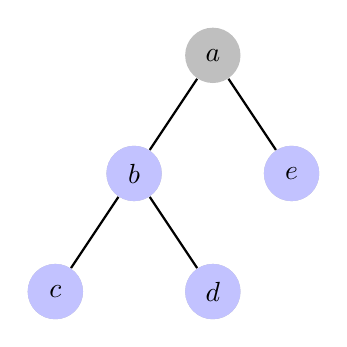
\begin{tikzpicture} [
                scale=1,
                vertex/.style={circle,fill=black!25,minimum size=20pt,inner sep=0pt},
                edge/.style = {draw,thick,-},
                selected vertex/.style = {vertex, fill=blue!24},
            ]
            \foreach \pos/\name in {
                    {(0,0)/c}, {(2,0)/d}, {(1,1.5)/b}, {(3,1.5)/e}, {(2,3)/a}}
                \node[vertex] (\name) at \pos {$\name$};
            \foreach \source/ \dest in {
                    b/c,b/d,a/b,a/e}
                \path[edge] (\source) edge (\dest);
            \foreach \vertex in {b,c,d,e}
                \path node[selected vertex] at (\vertex) {$\vertex$};
        \end{tikzpicture}
    \end{subfigure}
    \quad
    %%%%%%%%%%%%%%%%%%%%%%%%%%%%%%%%%%%%%%%%%%%%%%%%%%%%%%%%%%%%%%%%%%%%%%%%%%%%%%%%%%%%%
    \begin{subfigure}[b]{0.45\textwidth}
        \centering
        \caption{Sottografo (completo) indotto dai nodi dispari, e matching perfetto di costo minimo evidenziato}
        \label{fig:mchristmatching}
        \begin{tikzpicture} [
                scale=1,
                vertex/.style={circle,fill=black!25,minimum size=20pt,inner sep=0pt},
                edge/.style = {draw,thick,-},
                selected edge/.style = {draw,line width=5pt,-,blue!24},
            ]
            \foreach \pos/\name in {
                    {(0,0)/c}, {(2,0)/d}, {(1,1.5)/b}, {(3,1.5)/e}}
                \node[vertex] (\name) at \pos {$\name$};
            \foreach \source/ \dest in {
                    b/c,b/d,b/e,c/e,c/d,e/d}
                \path[edge] (\source) edge (\dest);
            \begin{pgfonlayer}{background}
                \foreach \source / \dest in {b/c,d/e}
                    \path[selected edge] (\source.center) -- (\dest.center);
            \end{pgfonlayer}
        \end{tikzpicture}
    \end{subfigure}
\end{figure}
    % \\[2pt]
% magic to split a figure https://tex.stackexchange.com/a/278748
\begin{figure}[htb]\ContinuedFloat
    \caption{Algoritmo di Christofides splittato in due pagine (cont.)}
    %%%%%%%%%%%%%%%%%%%%%%%%%%%%%%%%%%%%%%%%%%%%%%%%%%%%%%%%%%%%%%%%%%%%%%%%%%%%%%%%%%%%%
    \begin{subfigure}[b]{0.45\textwidth}
        \centering
        \caption{Ciclo Euleriano
            $ \langle c,b,d,e,a,b,c \rangle$
        }
        \label{fig:mchristeulertour}
        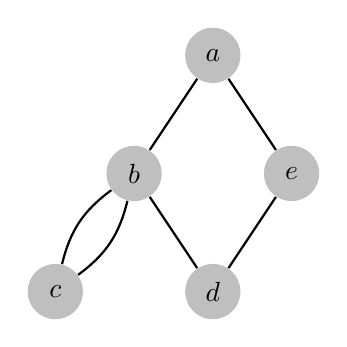
\begin{tikzpicture} [
                scale=1,
                vertex/.style={circle,fill=black!25,minimum size=20pt,inner sep=0pt},
                edge/.style = {draw,thick,-},
                bent right/.style = {bend right=20},
            ]
            \foreach \pos/\name in {
                    {(0,0)/c}, {(2,0)/d}, {(1,1.5)/b}, {(3,1.5)/e}, {(2,3)/a}}
                \node[vertex] (\name) at \pos {$\name$};
            \foreach \source/ \dest in {
                    b/d,a/b,a/e,d/e}
                \path[edge] (\source) edge (\dest);
            \foreach \source/ \dest in {
                    c/b,b/c}
                \path[edge] (\source) edge [bent right] (\dest);
        \end{tikzpicture}
    \end{subfigure}
    \quad
    %%%%%%%%%%%%%%%%%%%%%%%%%%%%%%%%%%%%%%%%%%%%%%%%%%%%%%%%%%%%%%%%%%%%%%%%%%%%%%%%%%%%%
    \begin{subfigure}[b]{0.45\textwidth}
        \centering
        \caption{Dopo lo \emph{shortcutting}:
            $ \langle c,b,d,e,a,\cancel{b},c \rangle$
        }
        \label{fig:mchristresult}
        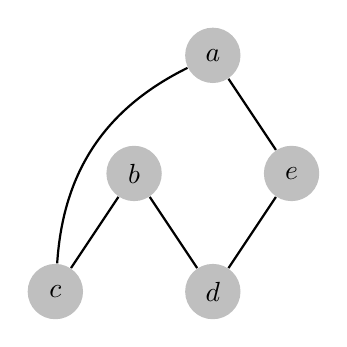
\begin{tikzpicture} [
                scale=1,
                vertex/.style={circle,fill=black!25,minimum size=20pt,inner sep=0pt},
                edge/.style = {draw,thick,-},
                bent right/.style = {bend right=30},
            ]
            \foreach \pos/\name in {
                    {(0,0)/c}, {(2,0)/d}, {(1,1.5)/b}, {(3,1.5)/e}, {(2,3)/a}}
                \node[vertex] (\name) at \pos {$\name$};
            \foreach \source/ \dest in {
                    b/d,a/e,d/e,b/c}
                \path[edge] (\source) edge (\dest);
            \foreach \source/ \dest in {
                    a/c}
                \path[edge] (\source) edge [bent right] (\dest);
        \end{tikzpicture}
    \end{subfigure}
\end{figure}

\lipsum{10}

\begin{figure}[h]
    \centering
    \caption{$3-CNF-SAT$ to $CLIQUE$}
    \label{fig:3cnfsatex}
    \begin{tikzpicture} [
            scale=1,
            vertex/.style={circle,fill=black!25,minimum size=20pt,inner sep=0pt},
            edge/.style = {draw,thin,-},
            outbound edge/.style = {draw,line width=4pt,-,blue!30},
            selected edge/.style = {draw,line width=4pt,-,red!30},
        ]
        % First we draw the vertices
        \foreach \pos/\name/\label in {
                % top left
                {(-1.5,5)/c/x_3},
                {(-2.5,3.5)/b/x_2},
                {(-3.5,2)/a/\bar{x_1}},
                % top right
                {(1.5,5)/d/x_1},
                {(2.5,3.5)/e/x_2},
                {(3.5,2)/f/\bar{x_3}},
                % bottom row
                {(2,0)/g/\bar{x_3}},
                {(0,0)/h/\bar{x_2}},
                {(-2,0)/i/x_1}}
            \node[vertex] (\name) at \pos {\name $\label$};
        % Connect vertices with edges
        \foreach \source/ \dest in {
                f/g,f/i,
                e/g,e/i,
                d/g,d/h,d/i,
                c/d,c/e,c/h,c/i,
                b/d,b/e,b/f,b/g,b/i,
                a/e,a/f,a/g,a/h}
            \path[edge] (\source) -- (\dest);
        % color some edges on background layer
        \begin{pgfonlayer}{background}
            \foreach \source / \dest in {c/d,d/i,i/c}
                \path[outbound edge] (\source.center) -- (\dest.center);
            \foreach \source / \dest in {a/e,e/g,g/a}
                \path[selected edge] (\source.center) -- (\dest.center);
        \end{pgfonlayer}
    \end{tikzpicture}
\end{figure}

\subsection{Parole in libertà}

Tutte le parole accentate si possono estrarre con

\texttt{grep -rEiohI '[a-z]*(à|è|é|ì|ò|ù)' | sort -u}

\begin{itemize}[noitemsep,parsep=0pt,partopsep=0pt,topsep=0pt]
    \item \texttt{-r}:
        Read all files under each directory, recursively
    \item \texttt{-E}:
        Interpret PATTERN as an extended regular expression
    \item \texttt{-i}:
        Ignore case distinctions in both the PATTERN and the input files
    \item \texttt{-o}:
        Print only the matched (non-empty) parts of a matching line
    \item \texttt{-h}:
        Suppress the prefixing of file names on output
    \item \texttt{-I}:
        Process a binary file as if it did not contain matching data
\end{itemize}

\texttt{sort -u} ordina l'output ed elimina i duplicati

affidabilità
andrà
associatività
avrà
Bé
biiettività
capacità
cardinalità
cioè
complessità
Complessità
così
difficoltà
Difficoltà
divisibilità
Divisibilità
dovrà
è
È
facilità
farà
finché
generalità
già
identità
Identità
inapprossimabilità
Inapprossimabilità
leggibilità
libertà
massimalità
metà
molteplicità
né
necessità
ottimalità
perché
Perché
però
più
polinomialità
potrà
primalità
probabilità
Probabilità
proprietà
Proprietà
pseudoprimalità
può
Può
qualità
quantità
randomicità
realtà
Riducibilità
sarà
sé
segnerà
Sì
soddisfacibilità
Soddisfacibilità
suriettività
transitività
unicità
Unicità
unità
utilità
validità
velocità
verità


\begin{figure}[h]
    \centering
    \caption{Unweighted graph}
    \label{fig:ug}
    \begin{tikzpicture} [
            auto,
            swap,
            scale=1.4,
            vertex/.style={circle,fill=black!25,minimum size=20pt,inner sep=0pt},
            selected vertex/.style = {vertex, fill=red!24},
            edge/.style = {draw,thick,-},
            weight/.style = {font=\small},
            selected edge/.style = {draw,line width=5pt,-,red!50},
            outbound edge/.style = {draw,line width=5pt,-,blue!50},
            ignored edge/.style = {draw,line width=5pt,-,black!20}
        ]
        % First we draw the vertices
        \foreach \pos/\name in {
                {(0,0)/A},
                {(0,2)/B},
                {(2,2)/C},
                {(4,2)/D},
                {(2,0)/E}}
            \node[vertex] (\name) at \pos {$\name$};
        % Connect vertices with edges and draw weights
        \foreach \source/ \dest in {
                B/C, C/E, C/D, D/E}
            \path[edge] (\source) -- (\dest);
        % color a node
        % \foreach \vertex in {B, D, E}
            % \path node[selected vertex] at (\vertex) {$\vertex$};
        \begin{pgfonlayer}{background}
            % \foreach \source / \dest in {B/C}
                % \path[outbound edge] (\source.center) -- (\dest.center);
            % \foreach \source / \dest in {D/G}
                % \path[selected edge] (\source.center) -- (\dest.center);
            % \foreach \source / \dest in {F/D}
                % \path[ignored edge] (\source.center) -- (\dest.center);
        \end{pgfonlayer}
    \end{tikzpicture}
\end{figure}

